% Format teze zasnovan je na paketu memoir
% http://tug.ctan.org/macros/latex/contrib/memoir/memman.pdf ili
% http://texdoc.net/texmf-dist/doc/latex/memoir/memman.pdf
% 
% Prilikom zadavanja klase memoir, navedenim opcijama se podešava 
% veličina slova (12pt) i jednostrano štampanje (oneside).
% Ove parametre možete menjati samo ako pravite nezvanične verzije
% mastera za privatnu upotrebu (na primer, u b5 varijanti ima smisla 
% smanjiti 
\documentclass[12pt,oneside]{memoir} 

% Paket koji definiše sve specifičnosti master rada Matematičkog fakulteta
\usepackage[latinica,biblatex]{matfmaster} 
%
% Podrazumevano pismo je ćirilica.
%   Ako koristite pdflatex, a ne xetex, sav latinički tekst na srpskom jeziku
%   treba biti okružen sa \lat{...} ili \begin{latinica}...\end{latinica}.
%
% Opicija [latinica]:
%   ako želite da pišete latiniciom, dodajte opciju "latinica" tj.
%   prethodni paket uključite pomoću: \usepackage[latinica]{matfmaster}.
%   Ako koristite pdflatex, a ne xetex, sav ćirilički tekst treba biti
%   okružen sa \cir{...} ili \begin{cirilica}...\end{cirilica}.
%
% Opcija [biblatex]:
%   ako želite da koristite reference na više jezika i umesto paketa
%   bibtex da koristite BibLaTeX/Biber, dodajte opciju "biblatex" tj.
%   prethodni paket uključite pomoću: \usepackage[biblatex]{matfmaster}
%
% Opcija [b5paper]:
%   ako želite da napravite verziju teze u manjem (b5) formatu, navedite
%   opciju "b5paper", tj. prethodni paket uključite pomoću: 
%   \usepackage[b5paper]{matfmaster}. Tada ima smisla razmisliti o promeni
%   veličine slova (izmenom opcije 12pt na 11pt u \documentclass{memoir}).
%
% Naravno, opcije je moguće kombinovati.
% Npr. \usepackage[b5paper,biblatex]{matfmaster}

% Pomoćni paket koji generiše nasumičan tekst u kojem se javljaju sva slova
% azbuke (nema potrebe koristiti ovo u pravim disertacijama)
\usepackage[latinica]{pangrami}
\usepackage[bottom]{footmisc}
\usepackage{listings}

\lstdefinestyle{customc}{
	belowcaptionskip=1\baselineskip,
	breaklines=true,
	frame=L,
	xleftmargin=\parindent,
	language=C,
	showstringspaces=false,
	basicstyle=\footnotesize\ttfamily,
	keywordstyle=\bfseries\color{green!40!black},
	commentstyle=\itshape\color{purple!40!black},
	identifierstyle=\color{blue},
	stringstyle=\color{orange},
	numbers=left,
	numberstyle=\tiny,
}

\lstdefinestyle{customasm}{
	belowcaptionskip=1\baselineskip,
	frame=L,
	xleftmargin=\parindent,
	language=[x86masm]Assembler,
	basicstyle=\footnotesize\ttfamily,
	commentstyle=\itshape\color{purple!40!black},
}


\lstdefinestyle{BashInputStyle}{
	language=bash,
	belowcaptionskip=1\baselineskip,
	basicstyle=\small\sffamily,
	numbers=left,
	numberstyle=\tiny,
	numbersep=3pt,
	frame=tb,
	columns=fullflexible,
	backgroundcolor=\color{yellow!20},
	linewidth=0.9\linewidth,
	xleftmargin=0.1\linewidth,
}

\lstdefinestyle{custombash}{
	belowcaptionskip=1\baselineskip,
	frame=L,
	xleftmargin=\parindent,
	language=[x86masm]Assembler,
	basicstyle=\footnotesize\ttfamily,
	commentstyle=\itshape\color{purple!40!black},
	backgroundcolor=\color{yellow!20},
	numbers=left,
	numberstyle=\tiny,
}

\lstset{escapechar=@,style=customc}

% Datoteka sa literaturom u BibTex tj. BibLaTeX/Biber formatu
\bib{DjordjeTodorovicMasterRad}

\newtheorem{primer}{Primer}

% Ime kandidata na srpskom jeziku (u odabranom pismu)
\autor{Đorđe Todorović}
% Naslov teze na srpskom jeziku (u odabranom pismu)
\naslov{Podrška za naprednu analizu promenljivih lokalnih za niti pomoću alata GNU GDB}
% Godina u kojoj je teza predana komisiji
\godina{2019}
% Ime i afilijacija mentora (u odabranom pismu)
\mentor{dr Milena \textsc{Vujošević-Janičić}, redovan profesor\\ Univerzitet u Beogradu, Matematički fakultet}
% Ime i afilijacija prvog člana komisije (u odabranom pismu)
\komisijaA{dr Filip \textsc{Marić}, redovan profesor\\ Univerzitet u Beogradu, Matematički fakultet}
% Ime i afilijacija drugog člana komisije (u odabranom pismu)
\komisijaB{dr Miroslav \textsc{Marić}, redovan profesor\\ Univerzitet u Beogradu, Matematički fakultet}
% Ime i afilijacija trećeg člana komisije (opciono)
% \komisijaC{}
% Ime i afilijacija četvrtog člana komisije (opciono)
% \komisijaD{}
% Datum odbrane (odkomentarisati narednu liniju i upisati datum odbrane ako je poznat)
% \datumodbrane{}

% Apstrakt na srpskom jeziku (u odabranom pismu)
\apstr{%

}

% Ključne reči na srpskom jeziku (u odabranom pismu)
\kljucnereci{Thread Local Storage, GNU‘s Not Unix, GNU Debugger, Datoteka jezgra}

\begin{document}
% ==============================================================================
% Uvodni deo teze
\frontmatter
% ==============================================================================
% Naslovna strana
\naslovna
% Strana sa podacima o mentoru i članovima komisije
\komisija
% Strana sa posvetom (u odabranom pismu)
\posveta{Daretu}
% Strana sa podacima o disertaciji na srpskom jeziku
%\apstrakt
% Sadržaj teze
\tableofcontents*

% ==============================================================================
% Glavni deo teze
\mainmatter
% ==============================================================================

% ------------------------------------------------------------------------------
\chapter{Uvod}
% ------------------------------------------------------------------------------

Softver je svuda oko nas, od automobila, aviona pa sve do kućnih aparata poput frižidera i šporeta. Veoma je važno da softver bude efikasan i kvalitetan. U težnji za efikasnijim softverom, kao i za softverom čija arhitektura oslikava logičku stukturu problema koriste se višenitne aplikacije. Da bi softver bio kvalitetan, u procesu razvoja neophodni su alati koji pomažu programeru da uoči i ispravi greške. Primer takvog alata je debager. Najpoznatiji debager je GNU GDB \cite{GDB}. Bitno je obezbediti laku analizu višenitnih programa, što je posebno izazovan zadatak.

Razvoj softvera za uređaje sa ugrađenim računarom (npr. softver za automobile) se obično odvija na ličnim računarima, jer uglavnom ugrađeni računari oskudevaju u pogledu resursa. Arhitektura procesora uređaja sa ugrađenim računarom se najčešće ne poklapa sa  arhitekturom procesora ličnih računara. Programi koji su prevedeni za jednu arhitekturu računara se ne mogu izvršavati na računarima drugačijih arhitektura. Greške u programima koji se izvršavaju na uređajima sa ugrađenim računarom najčešće otklanjamo koristeći alate na ličnim računarima.

Debager \emph{GNU GDB}, između ostalog, omogućava analiziranje i otklanjanje grešaka u programima koji se izvršavaju na računarima drugih arhitektura. Načini kroz koje se to može ostvariti jesu korišćenje \emph{GNU GDB} servera, uz korišćenje posebnih protokola, ili korišćenje datoteka jezgara.
Datoteka jezgra može biti kreirana iz korisničkog nivoa, npr. baš uz pomoć debagera \emph{GNU GDB}, ili prilikom neregularnog prekida izvršavanja programa samo jezgro operativnog sistema beleži informacije o stanju sistema i zapisuje je u nju. Datoteka jezgra sadrži stanje radne memorije procesa prilikom prekidanja rada programa na neki nestandardni način. Preciznije, ona sadrži informacije o vrednostima promenljivih, procesorskih registara, programskih brojača, informacije o samom procesu, informacije o nitima itd. Tako kreirana datoteka jezgra na gostujućoj arhitekturi može biti učitana i analizirana u debageru \emph{GNU GDB} na računaru sa arhitekturom domaćina.

Ovaj rad opisuje postupak korišćenja debagera prilikom dobijanja vrednosti promenljivih lokalnih za niti, ili, skraćeno, \emph{TLS} (eng. \emph{TLS-Thread Local Storage}) promenljivih \cite{TLS}. Definisanjem takvih promenljivih svaka nit ima različitu kopiju iste promenljive i prilikom analiziranja višenitnih programa značajno je pročitati vrednosti te promenljive iz svih niti. Ključna reč, programskih jezika \emph{C} i \emph{C++}, koja se dodaje ispred definicije ili deklaracije promenljive je \texttt{\_\_thread}. Različite arhitekture mogu imati različitu implementaciju \emph{TLS} mehanizma, te je njihovo čitanje iz debagera \emph{GNU GDB} dodatno otežano.
Glavni doprinos rada predstavlja omogućavanje čitanja vrednosti \emph{TLS} promenljive iz \emph{GNU GDB} za sve arhitekture procesora podržanih u debageru na arhitekturi domaćina, čime se proširuju dostupne informacije za analizu programa drugih arhitektura. Rezultati opisani u ovom radu su predstavljeni i na konfereniciji TELFOR \cite{TELFOR}.

Rad se pored prvog uvodnog, sastoji još iz pet poglavlja. Drugo poglavlje opisuje kako rade debageri. Navedena je podrška operativnih sistema i opis formata izvršnih fajlova koji omogućavaju rad debagera. Treće poglavlje pruža informacije o debageru \emph{GNU GDB} i opisuje detalje implementacije osnovnih komandi debagera. Četvrto poglavlje prikazuje detalje o \emph{TLS} promenljivama. Naveden je opis organizacije registara i memorije koji omogućavaju funkcionisanje \emph{TLS} mehanizma. Takođe je dat opis novih struktura podataka definisanih za promenljive lokalne za niti. U petom poglavlju je opisana implementacija poboljšanja debagera prilikom čitanja vrednosti promenljivih lokalnih za niti iz nedomaćinske datoteke jezgra, dok je u šestom poglavlju predstavljen zaključak rada.


% ------------------------------------------------------------------------------

\chapter{Kako rade debageri?}
\label{chp:debageri}

Greške su sastavni deo svakog rada koji obavlja čovek, te ih i programeri prave. Greške mogu biti hardverske i softverske. One mogu imati razne poslednice. Neke su manje važne, kao npr.~korisnički interfejs aplikacije ima neočekivanu boju pozadine. Postoje i greške koje mogu imati daleko veće posledice, pa čak i ugroziti živote drugih, kao npr.~greške u softveru ili hardveru uređaja i aplikacija avio industrije. Faza testiranja je veoma važna u ciklusu razvoja softvera. Nakon faze testiranja obično sledi faza analize i otklanjanja grešaka.

Debager (eng.~\emph{debagger}) je softverski alat koji koriste programeri za testiranje, analizu i otklanjanje grešaka u programima. Sam proces korišćenja takvih alata nazivamo debagovanjem (eng.~\emph{debugging}).
Debageri mogu pokrenuti rad nekog procesa ili se „nakačiti” na proces koji je već u fazi rada. U oba slučaja, debager preuzima kontrolu nad procesom. To mu mogućava da izvršava proces instrukciju po instrukciju, da postavlja tačke prekida (eng.~\emph{brakpoints}) itd. Proces izvršavanja programa od strane debagera sekvencijalno, instrukciju po instrukciju ili liniju po liniju, nazivamo koračanje. Tačke prekida su mogućnost debagera da zaustavi izvršavanje programa na određenoj tački. To može biti trenutak kada program izvrši određenu funkciju, liniju koda itd. Neki debageri imaju mogućnost izvršavanja funkcija programa koji se debaguje, uz ograničenje da program pripada istoj procesorskoj arhitekturi kao i domaćinski sistem na kojem se debager izvršava.

Podršku debagerima, u opštem slučaju, daju operativni sistemi, kroz sistemske pozive koji omogućavaju tim alatima da pokrenu i preuzmu kontrolu nad nekim drugim procesom. Za neke naprednije tehnike debagovanja poželjna je podrška od strane hardvera. U radu će detaljno biti obrađen rad \emph{UNIX}-olikih, posebno \emph{Linux} debagera. \emph{Windows} debageri i programski prevodioci ne prate standard \emph{DWARF} \cite{DWARF} prilikom baratanja sa debag informacijama. Alati za debagovanje u okviru operativnog sistema \emph{Windows} koriste standard \emph{Majkrosoft CodeView}.  Više informacija o ovom standardu može se pronaći u literaturi \cite{CodeView}.

\section{Prevođenje programa}

Programi koji se debaguju se prevode uz pomoć odgovarajuće opcije programskih prevodioca (za prevodioce \emph{GCC} \cite{GCC} i \emph{LLVM/Clang} \cite{LLVM}, to je opcija \texttt{-g}) koja obezbeđuje generisanje pomoćnih debag informacija. Ukoliko je program koji se analizira preveden bez optimizacija, debag informacije koje prate program su potpune. Za programe koji se puštaju u produkciju, da bi bili brži i zauzimali manje memorije, se prilikom prevođenja koriste optimizacije. Postoje različiti nivoi optimizacija i oni se zadaju kao opcija prevodiocu prilikom prevođenja. Nivoi optimizacija produkcijskih programa su \emph{-O2} i \emph{-O3}.

Prilikom optimizacija se gube razne debag informacije. Neke promenljive i funkcije programa neće biti predstavljene debag informacijama. Npr.~promenljiva programa može biti živa samo u nekim određenim delovima programa, pa programski prevodioci generišu debag informacije o njenim lokacijama samo u tim određenim delovima koda. Prilikom optimizacija na nivou mašinskog koda život promenljive može biti skraćen, pa čitanje vrednosti promenljive iz debagera u nekim sitacijama neće biti moguće, iako gledajući izvorni kod očekujemo da je ona živa u tom trenutku.

\section{Format DWARF}

\emph{DWARF} je debag fajl format koji se koristi od strane programskih prevodioca (kao npr.~\emph{GCC} ili \emph{LLVM/Clang}) i debagera (kao npr.~\emph{GNU GDB}) da bi se omogućilo debagovanje na nivou izvornog koda. Omogućava podršku za razne programske jezike kao što su \emph{C/C++} i \emph{Fortran}, ali je dizajniran tako da se lako može proširiti na ostale jezike. Arhitekturalno je nezavisan i predstavlja "most" između izvornog koda i izvršnog fajla. Trenutno je poslednji realizovani standard verzija 5 formata \emph{DWARF}.

Debag fajl format \emph{DWARF} na \emph{UNIX}-olike operativne sisteme, kao što su \emph{Linux} i \emph{MacOS}. Generisane debag informacije, prateći \emph{DWARF} standard, su podeljene u nekoliko sekcija sa prefiksom \texttt{.debug\_}. Neke od njih su \texttt{.debug\_line}, \texttt{.debug\_loc} i \texttt{.debug\_info} koje redom predstavljaju informacije o linijama izvornog koda, lokacijama promenljivih i ključna debag sekcija koja sadrži debag informacije koje referišu na informacije iz ostalih debag sekcija.
\emph{DWARF} je predstavljen kao drvolika struktura, smeštena u \texttt{.debug\_info} sekciju,  koja razne entitete programskog jezika opisuje osnovnom debag jedinicom \emph{DIE} (eng.~\emph{Debug Info Entry}). Osnovna debag jedinica može opisivati lokalnu promenljivu programa, formalni parametar, funkciju itd. Svaka od njih je identifikovana \emph{DWARF} tagom koji predstavalja informaciju o toj jedinici, gde je npr.~tag za lokalne promenljive predstavljen sa \texttt{DW\_TAG\_local\_variable}, ili tag za funkciju je obeležen sa \texttt{DW\_TAG\_subprogram}. Svaka debag jedinica je opisana određenim \emph{DWARF} atributima sa prefikosm \texttt{DW\_AT\_}. Oni mogu ukazivati na razne informacije o entitetu kao sto su ime promenljive ili funkcije, liniju deklaracije, itd. Koren svakog \emph{DWARF} stabla je predstavljen debag jedinicom, sa tagom  \texttt{DW\_TAG\_compile\_unit}, koja predstavlja kompilacionu jedinicu, tj. izvorni kod programa.

\begin{lstlisting} [style=customc, label={lst:c_kod}, caption={Primer programa napisanog u \emph{C} programskom jeziku.}]
#include <stdio.h>

int main()
{
  int x;
  x = 5;
  printf ("The value is %d\n", x);
  return 0;
}
\end{lstlisting}

Deo \emph{DWARF} stabla za primer \ref{lst:c_kod} programa napisanog u C programskom jeziku je prikazan u primeru \ref{lst:c_dwarf_stablo}.\newpage

\begin{lstlisting} [style=BashInputStyle, label={lst:c_dwarf_stablo}, caption={Primer \emph{DWARF} reprezentacije.}]
 <1><73>: Abbrev Number: 4 (DW_TAG_subprogram)
   <74>   DW_AT_external    : 1
   <74>   DW_AT_name        : (indirect string, offset: 0x68): main
   <78>   DW_AT_decl_file   : 1
   <79>   DW_AT_decl_line   : 3
   <7a>   DW_AT_type        : <0x57>
   <7e>   DW_AT_low_pc      : 0x400526
   <86>   DW_AT_high_pc     : 0x2a
   <8e>   DW_AT_frame_base  : 1 byte block: 9c         (DW_OP_call_frame_cfa)
   <90>   DW_AT_GNU_all_tail_call_sites: 1
 <2><90>: Abbrev Number: 5 (DW_TAG_variable)
   <91>   DW_AT_name        : x
   <93>   DW_AT_decl_file   : 1
   <94>   DW_AT_decl_line   : 5
   <95>   DW_AT_type        : <0x57>
   <99>   DW_AT_location    : 2 byte block: 91 6c      (DW_OP_fbreg: -20)
\end{lstlisting}

Funkcija \texttt{main} je predstavljena \emph{DWARF} tagom \texttt{DW\_TAG\_subprogram}. Atribut te debag jedinice predstavljen sa \texttt{DW\_AT\_name} ima vrednost imena funkcije. Atributi \texttt{DW\_AT\_low\_pc} i \texttt{DW\_AT\_high\_pc} redom predstavljaju adresu prve mašinske instrukcije te funkcije u memoriji programa i pomeraj na kojem se nalazi poslednja mašinska instrukcija te funkcije. Sledeći čvor drveta predstavlja promenljivu \texttt{x} istog test primera. Ta debag jedinica je dete čvora koji predstavlja funkciju \texttt{main} i ukazuje da se promenljiva \texttt{x} nalazi unutar funkcije \texttt{main}. Promenljiva \texttt{x} je predstavljena \emph{DWARF} tagom \texttt{DW\_TAG\_variable}. Atribut \texttt{DW\_AT\_name} predstavlja ime promenljive, \texttt{DW\_AT\_type} referiše na debag jedinicu koja predstavlja tip promenljive, dok \texttt{DW\_AT\_location} atribut predstavlja lokaciju promenljive u memoriji programa. 

\subsection{Debag promenljive}

Svaka promenljiva programa prevedenog sa debag informacijama, ukoliko se ne radi o optimizovanom programu, je predstavljena \emph{DWARF} tagom \texttt{DW\_TAG\_variable}. Atribut \texttt{DW\_AT\_location} ukazuje na lokaciju promenljive. Lokacija može biti predstavljena \emph{DWARF} izrazom, kao npr.~lokacija promenljive \texttt{x} prikazana sledećim primerom. \emph{DWARF} izraz te promenljive ukazuje da se ona nalazi na pomeraju \texttt{-20} trenutnog stek okvira \texttt{main} funkcije. U neoptimizovanom kodu sve promenljive imaju lokacije zadate \emph{DWARF} izrazom. Njihove vrednosti su dostupne debagerima u bilo kom delu koda u kom su definisane.

U optimizovanom kodu lokacija promenljive može sadržati referencu na informaciju o lokaciji u \texttt{.debug\_loc} sekciji. Lokacije u toj sekciji su predstavljene listama lokacija. Jedna promenljiva u optimizovanom kodu može biti smeštena na raznim memorijskim lokacijama ili registrima. Elementi liste opisuju lokacije promenljive na mestima u kodu gde je ona živa. Ukoliko promenljiva nije živa u nekom delu koda, programski prevodioci u optimizovanom kodu neće pratiti njenu lokaciju. Naredni primer \ref{lst:dwarf_var} predstavlja lokaciju promenljive u optimizovanom kodu.

\begin{lstlisting} [style=BashInputStyle, label={lst:dwarf_var}, caption={Primer \emph{DWARF} reprezentacije promenljive.}]
<2><90>: Abbrev Number: 5 (DW_TAG_variable)
<91>   DW_AT_name        : x
<93>   DW_AT_decl_file   : 1
<94>   DW_AT_decl_line   : 5
<95>   DW_AT_type        : <0x5e>
<99>   DW_AT_location    : 0x0 (location list)
\end{lstlisting}

Lokacijska lista promenljive \texttt{x} je predstavljena primerom \ref{lst:dwarf_loc}. U ovom konkretnom primeru, promenljiva živi samo na jednom mestu. Potencijalno je mogla imati još elemenata lokacijske liste. \texttt{Offset} predstavlja informaciju gde se lokacijska lista određene promenljive nalazi u \texttt{.debug\_loc} sekciji. \texttt{Begin} i \texttt{End} predstavljaju informaciju od koje do koje adrese u programu važi data lokacija, tj.~od koje do koje instrukcije je određena promenljiva živa. \texttt{Expression} predstavlja \emph{DWARF} izraz koji opisuje lokaciju promenljive.

\begin{lstlisting} [style=BashInputStyle, label={lst:dwarf_loc}, caption={Primer \emph{DWARF} reprezentacije lokacijske liste.}]
Contents of the .debug_loc section:
	Offset   Begin   End    Expression
	00000000 400450 40046a (DW_OP_fbreg: -20)
	0000001c <End of list>
\end{lstlisting}

%\section{Linux debageri}

\section{Format ELF}

\emph{ELF} (eng.~\emph{Executable and Linkable Format}) \cite{ELF} je format izvršnih fajlova, deljenih biblioteka, objektnih fajlova i datoteka jezgara.

\emph{ELF} sadrži razne informacije o samom fajlu. Podeljen je u dva dela: \emph{ELF} zaglavlje i podaci fajla. \emph{ELF} zaglavlje sadrži informacije o arhitekturi za koju je program preveden i definiše da li program koristi 32-bitni ili 64-bitni adresni prostor. Zaglavlje 32-bitnih programa je dužine 52 bajta, dok kod 64-bitnih programa zaglavlje je dužine 64 bajta. Podaci fajla mogu sadržati programsku tabelu zaglavlja (eng.~\emph{Program header table}), sekcijsku tabelu zaglavlja (eng.~\emph{Section header table}) i ulazne tačke prethodne dve tabele. Primer \ref{lst:elf} prikazuje \emph{ELF} fajl format počitan alatom \emph{readelf}:

\begin{lstlisting} [style=BashInputStyle, label={lst:elf}, caption={Primer \emph{ELF} zaglavlja.}]
ELF Header:
Magic:   7f 45 4c 46 02 01 01 00 00 00 00 00 00 00 00 00 
Class:                             ELF64
Data:                              2's complement, little endian
Version:                           1 (current)
OS/ABI:                            UNIX - System V
ABI Version:                       0
Type:                              EXEC (Executable file)
Machine:                           Advanced Micro Devices X86-64
Version:                           0x1
Entry point address:               0x400480
Start of program headers:          64 (bytes into file)
Start of section headers:          8992 (bytes into file)
Flags:                             0x0
Size of this header:               64 (bytes)
Size of program headers:           56 (bytes)
Number of program headers:         9
Size of section headers:           64 (bytes)
Number of section headers:         38
Section header string table index: 35
Section Headers:
...
\end{lstlisting}

U fajl formatu \emph{ELF} definisan je segment podataka koji sadrži informacije o globalnim promenljivama. Segment podataka je podeljen na dva dva dela. Tabela \ref{tab:elf_secs} opisuje \texttt{.bss} i \texttt{.data} sekcije. Sekcija \texttt{.bss} sadrži neinicijalizovane globalne promenljive, dok \texttt{.data} sadrži inicijalizovane. 

\begin{table}
	\begin{center}
		\begin{tabular}{ | l | p{5cm} | p{5cm} |}
			\hline
			\emph{Polje} & \emph{\texttt{.bss}} & \emph{\texttt{.data}} \\ \hline
			\texttt{sh\_name} & \texttt{.bss} & \texttt{.data} \\ \hline
			\texttt{sh\_type} & \texttt{SHT\_NOBITS} & \texttt{SHT\_PROGBITS} \\ \hline
			\texttt{sh\_flags} & \texttt{SHF\_ALLOC + SHF\_WRITE} & \texttt{SHF\_ALLOC + SHF\_WRITE} \\ \hline
			\texttt{sh\_addr} & Virtualna adresa sekcije & Virtualna adresa sekcije \\ \hline
			\texttt{sh\_offset} & Pomeraj sekcije & Pomeraj sekcije \\ \hline
			\texttt{sh\_size} & Veličina sekcije & Veličina sekcije \\ \hline
			\texttt{sh\_link} & \texttt{SHN\_UNDEF} & \texttt{SHN\_UNDEF} \\ \hline
			\texttt{sh\_info} & 0 & 0 \\ \hline
			\texttt{sh\_addralign} & Poravnanje sekcije & Poravnanje sekcije \\ \hline
			\texttt{sh\_entsize} & 0 & 0 \\ \hline
		\end{tabular}
	\end{center}
	\caption{\label{tab:elf_secs}Tabela vrednosti polja koji opisuju sekcije podataka.}
\end{table}

\section{Sistemski poziv \texttt{ptrace}}

Operativni sistem \emph{Linux} pruža sistemski poziv \texttt{ptrace} \cite{ptrace} koji debagerima omogućava rad. Ovaj sistemski poziv omogućava jednom procesu kontrolu nad izvršavanjem nekog drugog procesa, uključujući i menjanje njegove memorije i sadržaja registara.
Potpis ove funkcije je:
\newline\newline
\texttt{ long ptrace\newline(enum \_\_ptrace\_request request, pid\_t pid, void *addr, void *data);}
\newline

Prvi argument sistemskog poziva predstavlja informaciju kojom operativnom sistemu jedan proces, ne nužno debager, ukazuje na nameru preuzimanja kontrole drugog procesa. Ukoliko taj argument ima vrednost \texttt{PTRACE\_TRACEME} to ukazuje na nameru praćenja (eng.~\emph{tracing}) određenig procesa, \texttt{PTRACE\_PEEKDATA} i \texttt{PTRACE\_POKEDATA} redom ukazuju na nameru čitanja i pisanja  memorije, \texttt{PTRACE\_GETREGS} i \texttt{PTRACE\_SETREGS} se odnose na čitanje i pisanje registara. To su samo neki osnovni slučajevi korišćenja, za više informacija pogledati \cite{ptrace}. Drugi argument sistemskog poziva \texttt{pid} ukazuje na identifikacioni broj ciljanog procesa. Treći i četvrti argument se po potrebi koriste u zavisnosti od namere korišćenja sistemskog poziva \texttt{ptrace} za čitanje ili pisanje sa adrese datom trećim argumentom, pri tom baratajući podacima na adresi zadatoj četvrtim argumentom. To znači ukoliko se koristi \texttt{PTRACE\_TRACEME} poslednja tri argumenta sistemskog poziva se ignorišu. Ukoliko se koristi \texttt{PTRACE\_GETREGS} sa adrese \texttt{addr} se čita jedna reč iz memorije.

Navodimo par osnovnih primera korišćenja \texttt{ptrace} sistemskog poziva. Primeri 1 i 2 navode dva osnovna primera korišćenja \texttt{ptrace} sistemskog poziva. U nastavku teksta biće navedeno jos primera.

\begin{primer}
Program inicira da će biti praćen od strane roditeljskog procesa:

\texttt{ptrace(PTRACE\_TRACEME, 0, NULL, NULL);}
\end{primer}

\begin{primer}
Čitanje vrednosti registara procesa sa identifikatorom \texttt{8845} i upisivanje tih vrednosti na adresu promenljive \texttt{regs}:

\texttt{ptrace(PTRACE\_GETREGS, 8845, NULL, \&regs);}

\end{primer}

\section{Realizacija osnovnih elemenata upotrebe debagera}

U nastavku teksta se opisuju realizacije implementacije osnovnih elemenata upotrebe debagera.

\subsection{Tačke prekida}

Postoje dve vrste tačaka prekida (eng.~\emph{breakpoints}): softverske i hardverske \cite{GDB}.

Osvrnimo se prvo na softverske tačke prekida. Postavljanje tačaka prekida predstavlja jednu od najkorišćenijih mogućnosti debagera, te stoga navedimo par smernica kako je ista realizovana, u opštem slučaju. Ali takođe treba napomenuti da ne postoji jedinstveni poziv nekog sistemskog poziva za postavljanje tačke prekida, već se ista obavlja kao kombinacija više mogućnosti  sistemskog poziva \texttt{ptrace}. Opišimo ceo postupak na jednostavnom primeru.

Program je preveden za procesorsku arhitekturu \emph{Intel x86-64} i asemblerski k\^{o}d \texttt{main} funkcije je prikazan u primeru \ref{lst:asm}.\newpage
\begin{lstlisting} [style=customasm, label={lst:asm}, caption={Primer funkcije \texttt{main} u asemblerskom jeziku.}]
0000000000400450 <main>:
400450:       48 83 ec 08          sub    $0x8,%rsp
400454:       ba 05 00 00 00       mov    $0x5,%edx
400459:       be 04 06 40 00       mov    $0x400604,%esi
40045e:       bf 01 00 00 00       mov    $0x1,%edi
400463:       31 c0                xor    %eax,%eax
400465:       e8 c6 ff ff ff       callq  400430 <printf>
40046a:       31 c0                xor    %eax,%eax
40046c:       48 83 c4 08          add    $0x8,%rsp
400470:       c3                   retq   
400471:       66 2e 0f 1f 84       nopw   %cs:0x0(%rax,%rax,1)
400478:       00 00 00 
40047b:       0f 1f 44 00 00       nopl   0x0(%rax,%rax,1)

\end{lstlisting}


Primera radi, želimo da postavimo tačku prekida na treću po redu instrukciju funkcije \texttt{main}:

\texttt{be 04 06 40 00  mov \$0x400604, \%esi}

Da bismo to uradili, debager menja prvi bajt instrukcije sa posebnom magičnom vrednošću, obično \texttt{0xcc}, i kada izvršavanje dostigne do tog dela koda ono će se zaustaviti na tom mestu.

Pošto \texttt{0xbe} je zamenjeno sa \texttt{0xcc} i na tom mestu u kodu dobijamo instrukciju:

\texttt{cc 04 06 40 00  int3}

Ukoliko korisnik želi da nastavi dalje, instrukcija prekida se zamenjuje sa originalnom instrukcijom koja se izvršava i nastavlja se sa radom programa.

Instrukcija \texttt{int3} je posebna instrukcija procesorske arhitekture \emph{Intel x86-64}, koja izazva softverski prekid. Kada registar programski brojač (eng.~\emph{CPU register pc}) stigne do \texttt{int3} instrukcije izvršavanje se zaustavalja na toj tački. Debager je već upoznat od strane korisnika da je tačka prekida postavljena te on čeka na signal koji ukazuje na to da je program dostigao do instrukcije prekida. Operativni sistem prepoznaje instrukciju \texttt{int3}, poziva se specijalni obrađivač tog signala (na \emph{Linux} sistemima \texttt{do\_int3()}), koji dalje obaveštava debager šaljući mu signal sa kodom \texttt{SIGTRAP} koji on obrađuje na željeni način. Treba napomenuti da ovo važi za procesorsku arhitekturu \emph{Intel x86-64}, instrukcija prekida za arhitekture kao što su \emph{ARM, MIPS, PPC} itd., se drugačije kodira, ali postupak implementacije tačaka prekida je isti.

Ukoliko želimo da stavimo tačku prekida eksplicitno na funkciju \texttt{main}, za to koristimo posrednika u vidu \emph{DWARF} debag informacija. U tom slučaju debager traži element \emph{DWARF} stabla koji ukazuje na informacije o \texttt{main} funkciji, i odatle čita informaciju na kojoj adresi u memoriji se nalazi prva mašinska instrukcija date funkcije. Na primeru \ref{lst:main_sp} vidimo \emph{DWARF} element koji opisuje funkciju uz pomoć atributa. Debager će pročitati \texttt{DW\_AT\_low\_pc} atribut i na tu adresu postaviti \texttt{int3} instrukciju. Napomenimo da \emph{DWARF} debag simbole generišemo uz pomoć \texttt{-g} opcije kompajlera.
\begin{lstlisting} [style=BashInputStyle, label={lst:main_sp}, caption={Primer \emph{DWARF} reprezentacije funkcije \texttt{main}.}]
<1><73>: Abbrev Number: 4 (DW_TAG_subprogram)
  <74>   DW_AT_external    : 1
  <74>   DW_AT_name        : (indirect string, offset: 0x68): main
  <78>   DW_AT_decl_file   : 1
  <79>   DW_AT_decl_line   : 3
  <7a>   DW_AT_type        : <0x57>
  <7e>   DW_AT_low_pc      : 0x400526
  <86>   DW_AT_high_pc     : 0x2a
  <8e>   DW_AT_frame_base  : 1 byte block: 9c
  <90>   DW_AT_GNU_all_tail_call_sites: 1
\end{lstlisting}

Hardverske tačke prekida su direktno povezane sa hardverom u vidu specijalnih registara. Postavlja se na određenu adresu i hardverski \emph{watchpoint} monitori za zadatu adresu mogu signalizirati razne promene, npr. čitanje, pisanje ili izvršavanje, što im daje prednost u odnosu na softverske tačke prekida. Mane u odnosu na softverske tačke prekida su performanse, koje su neuporedivo sporije, i takođe neophodna hardverska podrška za korišćenje hardverskih tačaka prekida.

\subsection{Koračanje}

Pod procesom koračanja (eng.~\emph{stepping}) kroz program podrazumevamo izvršavanje programa sekvencu po sekvencu. Sekvenca može biti jedna procesorska instrukcija, linija koda ili pak neka funkcija programa koji se debaguje \cite{GDB}.

Instrukcijsko koračanje na platformi Intel x86-64 je direktno omogućeno kroz sistemski poziv \texttt{ptrace}:\newline
\texttt{ptrace(PTRACE\_SINGLESTEP, debuggee\_pid, nullptr, nullptr);}
\newline

Operativni sistem će poslati debageru signal \texttt{SIGTRAP} kada je korak izvršen.

Pored instrukcijkog koračanja pomenućemo još jednu vrstu koračanja u neku funkciju koja je pozvana \texttt{call} ili \texttt{jump} instrukcijom. Komanda debagara \emph{GNU GDB} koja nam to omogućava jeste \texttt{step in}.

Treba napomenuti da postoje arhitekture za koje ovo ne važi, kao npr. platforma \emph{ARM}, koja nema hardversku podršku za instrukcijsko koračanje i za njih se koračanje implementira na drugačiji način, uz pomoć emulacije instrukcija, ali u ovom radu neće biti reči o tome.

\subsection{Izlistavanje pozivanih funkcija}

Objasnimo komandu izlistavanje pozivanih funkcija (eng.~\emph{backtrace}) posmatrajući organizaciju stek okvira (eng.~\emph{stack frames}) na platformi Intel x86-64 \cite{GDB}.

\begin{figure}[h!]
	\begin{center}
		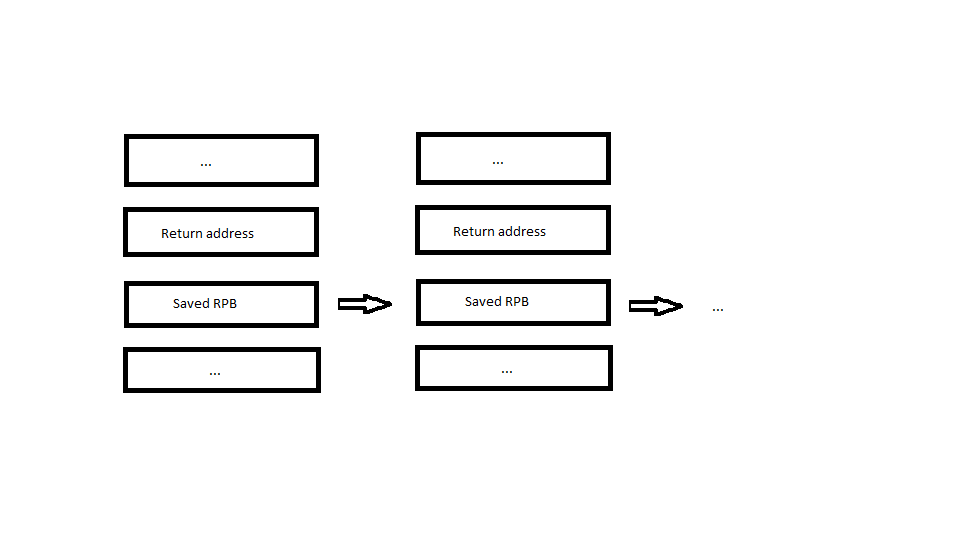
\includegraphics[scale=0.6]{slike/stack_frame.png}
	\end{center}
	\caption{Primer ređanja stek okvira na x86-64 platformi.}
	\label{fig:stack}
\end{figure}

Na slici \ref{fig:stack} navedeni su stek okviri za dva funkcijska poziva. Pre povratne vrednosti funkcije obično se ređaju argumenti funkcije. Sačuvana adresa u registru \texttt{RBP} jeste adresa stek okvira svog pozivaoca. Prateći sve okvire kao elemente povezane liste dolazimo do svih pozivanih funkcija do zadate tačke. Ako se pitamo kako debager ima informaciju o imenu funkcije odgovor je u tome što pretražuje DWARF stablo sa debag informacijama, tražeći \texttt{DW\_TAG\_subprogram} sa odgovarajućom povratnom adresom, pritom čitajući \texttt{DW\_AT\_name} atribut tog elementa.

\subsection{Čitanje vrednosti promenljivih}

Za čitanje vrednosti promenljivih u programu, debager pretražuje DWARF stablo tražeći promenljivu sa zadatim imenom. U slučaju lokalnih promenljivih, traži se \texttt{DW\_TAG\_variable} element čiji \texttt{DW\_AT\_name} odgovara navedenoj promenljivoj. Kada se ista pronađe konsultuje se \texttt{DW\_AT\_location}, koji ukazuje na lokaciju gde se vrednost promenljive nalazi. Ukoliko ovaj atribut nije naveden debager će vrednost takve promenljive smatrati kao optimizovanu prijavljujući informaciju o tome \cite{GDB}.

\chapter{Debager GNU GDB}
\label{chp:GDB}

\emph{GNU GDB} je alat koji omogućava uvid u događanja unutar drugog programa koji se nalazi u fazi izvršavanja, ili u slučaju neregularnog prekida izvršavanja programa uvid u to šta se dešavalo pa je do toga došlo. \emph{GNU GDB} debager takođe omogućava uvid u to šta se dešavalo sa programima i na platformama koje imaju različitu arhitekturu od domaćinske arhitekture (eng.~\emph{host architecture}). Da bi se to realizovalo koristi se \emph{GNU GDB} server, što se naziva udaljeno debagovanje, jer se udaljenom uređaju pristupa preko posebnih protokola. U svrhe debagovanja programa drugih procesorskih arhitektura na domaćinskim platformama se takođe upotrebljava \emph{Multiarch GNU GDB} koji koristi biblioteke namenjene ciljanim arhitekturama. Programi koji mogu biti analizirani mogu biti napisani u raznim programskim jezicima, kao što su \emph{Ada, C, C++, Objective-C, Pascal}. \emph{GNU GDB} debager se može pokrenuti na najpopularnijim operativnim sistemima \emph{UNIX} i \emph{Microsoft Windows} varijanti. U radu se podrazumeva korišćenje \emph{UNIX}-olikog operativnog sistema.

\section{Istorija \emph{GNU GDB} debagera}

Izvorni kod alata \emph{GNU GDB} je originalno napisan od strane Ričarda Stolmana 1986. godine kao deo \emph{GNU} sistema \cite{GDBDOC}. \emph{GNU GDB} je slobodan i besplatan softver realizovan pod \emph{GNU General Public License (GPL)}. Od 1990.~do 1993.~godine alat je održavao Džon Gilmor, a trenutno za održavanje alata je zadužena \emph{GDB Steering Committee} grupa, odobrena od strane \emph{FSF} (eng.~\emph{Free Software Foundation}) \cite{FSF}.

Poslednja realizovana verzija alata \emph{GNU GDB} je 8.2.1.

\section{Šta je \emph{arhitektura} za GNU GDB?}

Za debager \emph{GNU GDB} arhitektura je veoma labav koncept. Može se posmatrati kao bilo koje svojstvo programa koji se debaguje, ali obično se misli na procesorsku arhitekturu. Za debager su bitna dva svojstva procesorske arhitekture:

\begin{itemize}
	\item Skup instrukcija (eng.~\emph{Instruction Set Architecture - ISA}) predstavlja specifičnu kombinaciju registara i mašinskih instrukcija.
	\item ABI (eng.~\emph{Application Binary Interface}) predstavlja spisak pravila koja propisuju pravilan način korišćenja skupa instrukcija.
\end{itemize}

\subsection{Domaćinski GNU GDB}

Domaćinski \emph{GNU GDB} je preveden za istu procesorsku arhitekturu kao i računar na kome se alat izvršava. Korišćenje domaćinskog \emph{GNU GDB} nad nekim programom ima ograničenje. Program koji se debaguje mora biti iste procesorske arhitekture kao i arhitektura domaćina.

\subsubsection{Prevođenje domaćinskog GNU GDB debagera}

Preuzimanje izvornog koda debagera se vrši komandama prikazanim na \ref{lst:preuzimanje}.
\begin{lstlisting} [style=BashInputStyle, label={lst:preuzimanje}, caption={Komande korišćene za preuzimanje izvornog koda debagera.}]
mkdir gdb
cd gdb
git pull http://gnu.org/gnu/gdb.git

\end{lstlisting}

\emph{ Prva komanda pravi direktorijum u kome se izgrađuje (prevodi) alat. Druga komanda vrši pozicioniranje trenutne putanje u taj direktorijum. Trećom komandom se preuzima izvorni kod alata.}\newpage

Prvi korak prevođenja je konfiguracija direktorijuma u kome se prevođenje izvršava. Komandama sa \ref{lst:makefile} se kreira \texttt{Makefile}.
\begin{lstlisting} [style=BashInputStyle, label={lst:makefile}, caption={Komande korišćene za kreiranje \texttt{Makefile}.}]
mkdir build
cd build
../configure

\end{lstlisting}
\emph{Prva komanda pravi direktorijum u kome se izgrađuje (prevodi) alat. Druga komanda vrši pozicioniranje trenutne putanje u taj direktorijum. Trećom komandom se kreira \texttt{Makefile}. Skripte \texttt{configure} kao ulaz parsiraju \texttt{Makefile.in} skriptu podešavajući okruženje (putanje do deljenih biblioteka, programski prevodilac i drugo) prilikom čega je krajnji izlaz fajl \texttt{Makefile} kojim se izgrađuje (prevodi) softver.}

Nakon konfiguracije direktorijuma prevođenje alata se vrši komandom:
\begin{lstlisting} [style=BashInputStyle, label={lst:make}, caption={Izvršavanje komande \texttt{make}}.]
make
\end{lstlisting}

\subsubsection{Pokretanje domaćinskog GNU GDB debagera}

\emph{GNU GDB} očekuje kao argument komandne linije program koji je preveden za istu procesorsku arhitekturu. Ukoliko je trenutna putanja pozicionirana u direktorijum gde je izgrađen alat, pokretanje alata nad programom pod imenom \emph{test} se vrši sledećom komandom prikazanom na \ref{lst:pokretanje}.
\begin{lstlisting} [style=BashInputStyle, label={lst:pokretanje}, caption={Pokretanje debagera.}]
./gdb/gdb test

\end{lstlisting}


\subsubsection{Korišćenje domaćinskog GNU GDB debagera}

Pokažimo neke od osnovnih komandi debagera \emph{GNU GDB}.

Primer programa koji se debaguje je prikazan na \ref{lst:c_primer_dbg}.\newpage

\begin{lstlisting} [style=customc, label={lst:c_primer_dbg}, caption={Primer programa u programskom jeziku C.}]
int fn1 (int &addr) {
  return 0;
}

int main()
{
  int a = 5;
  fn1(&a);
}
\end{lstlisting}

\begin{description}

\item{\emph{Postavljanje tačke prekida}}

Postavljanje tačke prekida na funkciju programa koji se debaguje se vrši komandom \texttt{break}. Program koji se debaguje se zaustavlja kada dostigne do određene funkcije. Primer korišćenja postavljanja tačke prekida na funkciju (u ovom slučaju \texttt{fn1}) je prikazan na \ref{lst:break}.

\begin{lstlisting} [style=BashInputStyle, label={lst:break}, caption={Primer postavljanja tačke prekida.}]
(gdb) break fn1
Breakpoint 1 at 0x4005fe: file test.c, line 4.
(gdb) r
Starting program: /master_examples/x86_arch/test 
7
Breakpoint 1, fn1 (arg=0x7fffffffdbf4) at test.c:4
4		(*arg)++;
\end{lstlisting}

\item{\emph{Izvršavanje programa sekvencu po sekvencu}}

Izvršavanje programa sekvencu po sekvencu se radi pomoću tehnike koračanja. Komanda u okviru debagera \emph{GNU GDB} koja nam omogućava izvršavanje instrukciju po instrukciju je \texttt{stepi}. Primer korišćenja komande \texttt{stepi}, uz pomoć korišćenja komande \texttt{disassemble} koja nam prikazuje asemblerski kod programa koji se debaguje je prikazan na \ref{lst:dis}.\newpage

\begin{lstlisting} [style=BashInputStyle, label={lst:dis}, caption={Primer korišćenja komande \texttt{stepi}.}]
(gdb) disassemble
Dump of assembler code for function fn1:
0x00000000004005f6 <+0>:	push   %rbp
0x00000000004005f7 <+1>:	mov    %rsp,%rbp
0x00000000004005fa <+4>:	mov    %rdi,-0x8(%rbp)
=> 0x00000000004005fe <+8>:	mov    -0x8(%rbp),%rax
0x0000000000400602 <+12>:	mov    (%rax),%eax
0x0000000000400604 <+14>:	lea    0x1(%rax),%edx
0x0000000000400607 <+17>:	mov    -0x8(%rbp),%rax
0x000000000040060b <+21>:	mov    %edx,(%rax)
0x000000000040060d <+23>:	mov    -0x8(%rbp),%rax
0x0000000000400613 <+29>:	cmp    $0x5,%eax
0x0000000000400616 <+32>:	jle    0x400627 <fn1+49>
0x0000000000400628 <+38>:	pop    %rbp
0x0000000000400629 <+42>:	retq   
End of assembler dump.
(gdb) stepi
0x0000000000400602	4		(*arg)++;
(gdb) disassemble 
Dump of assembler code for function fn1:
0x00000000004005f6 <+0>:	push   %rbp
0x00000000004005f7 <+1>:	mov    %rsp,%rbp
0x00000000004005fa <+4>:	mov    %rdi,-0x8(%rbp)
0x00000000004005fe <+8>:	mov    -0x8(%rbp),%rax
=> 0x0000000000400602 <+12>:	mov    (%rax),%eax
0x0000000000400604 <+14>:	lea    0x1(%rax),%edx
0x0000000000400607 <+17>:	mov    -0x8(%rbp),%rax
0x000000000040060b <+21>:	mov    %edx,(%rax)
0x000000000040060d <+23>:	mov    -0x8(%rbp),%rax
0x0000000000400613 <+29>:	cmp    $0x5,%eax
0x0000000000400616 <+32>:	jle    0x400627 <fn1+49>
0x0000000000400628 <+38>:	pop    %rbp
0x0000000000400629 <+42>:	retq   
End of assembler dump.
\end{lstlisting}

Izvršavanje sledeće linije programa se radi korišćenjem komande \texttt{next}. Primer korišćenja \texttt{next} komande je prikazan na \ref{lst:next}.

\begin{lstlisting} [style=BashInputStyle, label={lst:next}, caption={Primer korišćenja komande \texttt{next}.}]
(gdb) r
The program being debugged has been started already.
Start it from the beginning? (y or n) y
Starting program: /master_examples/x86_arch/test 
4
Breakpoint 1, fn1 (arg=0x7fffffffdbf4) at test.c:4
4		(*arg)++;
(gdb) next
5	    if ((*arg) > 5)
\end{lstlisting}

\end{description}


\section{Datoteke jezgra}

Datoteka jezgra (eng.~\emph{core dump file}) je snimak (eng.~\emph{snapshot}) memorije programa, registara i ostalih sistemskih informacija u trenutku neočekivanog prekida rada programa. Veoma važnu ulogu ima u procesu debagovanja programa sa uređaja sa ugrađenim računarom koji često pripadaju različitoj procesorskoj arhitekturi u odnosu na lični računar. Ugrađeni uređaji obično imaju ograničene resurse, pa često na takvim platformama ne postoji debager. Najčešća procedura debagovanja ovakvih programa jeste prebacivanje datoteke jezgra i programa na lični računar na kome se analiza problema odvija koristeći debager.

\subsection{Struktura datoteke jezgra}

Datoteke jezgra sadrže razne informacije iz memorije programa uključujući i vrednosti lokalnih promenljivih, globalnih promenljivih, podatke lokalne za niti itd. Takođe sadrži vrednosti registara u trenutku prekida programa. U to spadaju i programski brojač i stek pokazivač.

Sadržaj datoteke jezgra je organizovan sekvencijalno sledećim redosledom:

\begin{description}
	\item[Zaglavlje.]
	Sadrži osnovne informacije o datoteci jezgra i pomeraje (eng.\emph{~offset}) kojima se lociraju ostale informacije iz nje.
	\item[\texttt{ldinfo} strukture.]   
	Definiše informacije relevantne za dinamički loader.
	\item[\texttt{mstsave} strukture.]
	Definiše informacije relevantne za sistemske niti.
	\item[Korisnički stek.]
	Sadrži kopiju korisničkog steka u trenutku neregularnog prekida rada programa.
	\item[Segment podataka.]   
	Sadrži kopiju segmenta podataka u trenutku pucanja programa.
	\item[Memorijski mapirani regioni]\footnote{Memorija programa je podeljena u nekoliko memorijskih regiona. Maprianjem memorijskih regiona se čuvaju relacije između virtualnih i fizičkih adresa programa.} \textbf{i \texttt{vm\_info} strukture.}
	Sadrži informacije o pomerajima i dužinama mapiranih regiona.
\end{description}

\subsection{Generisanje datoteke jezgra}

Datoteke jezgra se generišu ukoliko dođe do neregularnog prekida programa. To je podrazumevana akcija prilikom pojave signala operativnog sistema koji ukazuju na prekid rada programa. Jezgra \emph{UNIX}-olikih operativnih sistema podrazumevano postavljaju dužinu datoteka jezgara na \texttt{0}. To je razlog zašto na našim sistemima nemamo datoteku jezgra nakon npr.~prekidanja programa uz poruku \emph{Segmentation fault}. Da bi se datoteke jezgra generisale, potrebno je eksplicitno promeniti dužinu datoteka jezgara koristeći komandu prikazanu na \ref{lst:unlimited}.

\begin{lstlisting} [style=BashInputStyle, label={lst:unlimited}, caption={Primer korišćenja komande \texttt{unlimited}.}]
ulimit -c unlimited

\end{lstlisting}

Datoteka jezgra se može generisati i iz korisničkog nivoa koristeći debager \emph{GNU GDB} komandom \texttt{gcore}.

\section{\emph{Multiarch} GNU GDB}

\emph{Multiarch GNU GDB} je verzija debagera koja može da debaguje programe sa platformi različitih arhitektura. Alat na korisničkom nivou emulira instrukcije i registre ciljanih platformi. Potrebne su mu i deljene biblioteke za tu ciljanu platformu koje koristi program koji se debaguje. Skup komandi alata je limitiran u odnosu na domaćinski \emph{GNU GDB}.

\subsection{Prevođenje \emph{Multiarch} GNU GDB}

Prvi korak je pozicioniranje u direktorijum sa izvornim kodom debagera je prikazan na \ref{lst:cd}.
\begin{lstlisting} [style=BashInputStyle, label={lst:cd}, caption={Pozicioniranje u direktorijum \emph{gdb}.}]
cd gdb

\end{lstlisting}

Sledeći korak je konfiguracija direktorijuma u kome se prevođenje izvršava. Ovim komandama kreiramo \texttt{Makefile} kojim odobravamo debagovanje svih podržanih arhitektura u alatu GBD (kao npr.~\emph{MIPS32, MIPS64, ARM, AARCH64, x86\_64, i386, SPARC}) je prikazan na \ref{lst:mkdir}.

\begin{lstlisting} [style=BashInputStyle, label={lst:mkdir}, caption={Konfiguracija direktorijuma za izgradnju debagera.}]
mkdir build_multi
cd build_multi
../configure --enable-targets=all

\end{lstlisting}
\emph{Prva komanda pravi direktorijum u kome se izgrađuje (prevodi) alat. Druga komanda vrši pozicioniranje trenutne putanje u taj direktorijum. Trećom komandom se kreira \texttt{Makefile}. Pošto je prilikom konfiguracije navedena opcija \texttt{--enable-targets=all} time je omogućeno prevođenje alata za sve podržane arhitekture. Takođe je moguće konfigurisati prevođenje za samo određene arhitekture navodeći eksplicitno opciju kojom se navode ciljane procesorske arhitekture, npr.~\texttt{–enable-targets=mips-linux-gnu} za arhitekturu \emph{MIPS} ili \texttt{–enable-targets=arm-linux-gnu} za arhitekturu \emph{ARM}. Osnovna razlika između \texttt{Makefile}-ova domaćinske i \texttt{Multiarch} verzije debagera je ta što je za domaćinski alat potrebno okruženje (deljene biblioteke, programski prevodilac, itd.) samo za domaćinsku arhitekturu. Za \texttt{Multiarch} verziju alata potrebno je pronaći putanje do programskog prevodioca i deljenih biblioteka za ciljane platforme navedene opcijom \texttt{--enable-targets=}. Ukoliko konfiguracione skripte ne pronađu ciljano okruženje za neku od navedenih arhitektura, ta će biti ignorisana.}

\subsection{Pokretanje \emph{Multiarch} GNU GDB}

Ukoliko je trenutna putanja pozicionirana u direktorijum gde je izgrađen alat, pokretanje alata \emph{Multiarch} GDB nad programom pod imenom \emph{test} se vrši na isti način kao i domaćinska verzija debagera komandom prikazanom na \ref{lst:pokretanjee}.
\begin{lstlisting} [style=BashInputStyle, label={lst:pokretanjee}, caption={Pokretanje debagera.}]
./gdb/gdb test

\end{lstlisting}

\subsection{Korišćenje \emph{Multiarch} GNU GDB}

Spisak komandi koje se mogu koristiti korišćenjem \emph{Multiarch} verzije debagera \emph{GNU GDB} je limitiran. To se odnosi na izvršavanje programa koji se debaguje, jer program pripada drugačijem adresnom prostoru. Neke od komandi koje mogu biti upotrebljene su izlistavanje vrednosti registara programa, izlistavanje instrukcija, analiza stek okvira pozivanih funkcija, itd. Najčešće se ova verzija alata koristi tako što se učita datoteka jezgra koja je generisana na ciljanoj platformi kada je program koji se debaguje neočekivano prekinuo sa radom. To obično prati analiza uzroka greške.

\subsubsection{Primer učitavanja datoteke jezgra u debager GNU GDB}

U primeru \ref{lst:core-file} je prikazano učitavanje datoteke jezgra programa čije izvršavanje je prekinuto od strane jezgra operativnog sistema. Komandom alata \texttt{core-file} se učitava datoteka jezgra u debager. Da bi se izazvalo generisanje datoteke jezgra u izvornom kodu programa napisanog u \emph{C} ili \emph{C++} programskom jeziku može se koristiti \texttt{abort()} funkcija iz standardne \emph{C} biblioteke. U primeru ispod je pozvana ta funkcija koja je izazvala prekid programa uz signal \texttt{SIGABRT}. Tom prilikom jezgro operativnog sistema je napravilo datoteku jezgra sa imenom \emph{core}.
\begin{lstlisting} [style=BashInputStyle, label={lst:core-file}, caption={Primer korišćenja komande \texttt{core-file}.}]
(gdb) core-file core
[New LWP 20586]
[Thread debugging using libthread_db enabled]
Using host libthread\_db library "/lib/x86-linux-gnu/libthread_db.so.1".
Core was generated by `./test.core'.
Program terminated with signal SIGABRT, Aborted.
#0  0x00007fb229164428 in raise (sig=6) at raise.c:54
\end{lstlisting}


U primeru \ref{lst:bt} je prikazana upotreba komande debagera \emph{GNU GDB} \texttt{bt}. Ona se koristi za izlistavanje pozivanih funkcija programa. Stek okviri programa koji su prikazani na primeru potvrđuju da je u funkciji \texttt{main()} došlo do poziva \texttt{abort()} funkcije. Što je izazvalo prekid rada programa.

\begin{lstlisting} [style=BashInputStyle, label={lst:bt}, caption={Primer korišćenja komande \texttt{bt}.}]
(gdb) bt
#0  0x00007fb229164428 in raise (sig=6) at raise.c:54
#1  0x00007fb22916602a in abort () at abort.c:89
#2  0x0000000000400605 in main () at tls.c:18
\end{lstlisting}

\subsubsection{Analiza datoteke jezgra}

U primeru \ref{lst:core2} je prikazan primer korišćenja debagera \emph{Multiarch GNU GDB} prilikom učitavanja datoteke jezgra generisane na uređaju sa ugrađenim računarom arhitekture \emph{MIPS}. Uz datoteku jezgra učitavaju se izvršni fajl i deljene biblioteke koje izvršni fajl koristi na ciljanoj platfomi.


\begin{lstlisting} [style=BashInputStyle, label={lst:core2}, caption={Primer učitavanja datoteke jezgra generisane na uređaju sa ugrađenim računarom arhitekture \emph{MIPS}.}]
(gdb) set solib-search-path ~/master_examples/mips_arch/
(gdb) core-file ~/master_examples/mips_arch/core
[New LWP 21808]
[New LWP 21813]
[New LWP 21810]
[New LWP 21809]
[New LWP 21811]
[New LWP 21812]
Core was generated by `example'.
Program terminated with signal SIGABRT, Aborted.
#0  0x00000000 in ?? ()
[Current thread is 1 (LWP 21808)]
\end{lstlisting}

Komanda \texttt{set solib-search-path \emph{dir}} debagera \emph{GNU GDB} korišćena u prethodnom primeru služi za navođenje direktorijuma iz kojeg debager treba da koristi deljene biblioteke za učitani program. Ta komanda je veoma bitna za debagovanje programa sa platformi drugih arhitektura, jer ukoliko putanja nije navedena debager koristi biblioteke na domaćinskoj mašini.

U primeru \ref{lst:inforeg} je prikazana upotreba komande \texttt{info registers}. \emph{Multiarch GNU GDB} čita informaciju o arhitekturi programa koji se debaguje iz datoteke jezgra. Nakon toga čita vrednosti registara iz datoteke i ispisuje ih na standardni izlaz.

\begin{lstlisting} [style=custombash, label={lst:inforeg}, caption={Primer korišćenja komande \texttt{info registers}.}]
(gdb) info registers 
	 zero      at       v0     v1       a0	        a1       
R0   00000000 00005530 00000000 00005530 00000000 00005530
       t0       t1       t2       t3       t4       t5       
R8   00000000 00000000 00000000 7fcf4ca0 00000000 00000000
       s0       s1       s2       s3       s4       s5       
R16  00000000 7719a684 00000000 00000000 00000000 00000002
          k0       k1       gp       sp        s8      ra
R24   00000000 771c6490 00000000 77160634  00000000 7fcf4c20
       sr       lo       hi      bad      cause       pc
     00000000 00000000 77165000 00000000 00b24608 00000000 
       fsr      fir
     00000000 00000000
\end{lstlisting}

\chapter{Promenljive lokalne za niti}
\label{chp:TLS}

% ------------------------------------------------------------------------------
Pisanje višenitnih programa predstavlja fudamentalan i neizbežan koncept savremenog programiranja. Gotovo nijedan kompleksan korisnički program ne može biti napisan bez korišćenja niti. Preciznije, niti podižu performanse i brzinu programa, te se sve češće koriste u pisanju softvera. Promenljive lokalne za niti su važan mehanizam koji se koristi u okviru višenitnih aplikacija programskih jezika \emph{C} i \emph{C++}. One omogućavaju definisanje promenljivih koje imaju različitu vrednost u svakoj niti. Jedan primer je promenljiva koja jednoznačno identifikuje grešku koja je nastala u programu. Greška može biti izazvana u svakoj posebnoj niti iz različitog razloga, te promenljiva koja je opisuje treba da ima različitu vrednost u svakoj niti.

\section{Uvod u \emph{TLS}}

Povećanje korišćenja niti u programiranju dovelo je do potrebe programera za boljim načinom rukovanja podacima lokalnim za niti. Skup interfejsa za rukovanje nitima \emph{POSIX} \cite{POSIX} omogućava kreiranje istog void * objekata posebno za svaku nit. Taj interfejs je nezgrapan za korišćenje, jer objekat mora biti dinamčki alociran u vremenu izvršavanja programa. Kada se objekat više ne koristi, mora da se oslobodi. Celokupan proces zahteva dosta posla programera. Pored toga, podložan je greškama. Iz tih razloga postoji potreba za efikasnijim rešenjem. Da bi se odgovorilo na opisane probleme, odlučeno je da se programski jezici prošire i tako prepuste težak posao programskim prevodiocima.

Za jezike \emph{C} i \emph{C++} ključna reč \texttt{\_\_thread} se koristi za deklaraciju i definiciju promenljivih lokalnih za niti. Neki primeri deklaracija promenljivih lokalnih za niti su prikazani u okviru listinga \ref{lst:deklaracije}. Od \emph{C++11} verzije jezika koristi se i ključna reč \texttt{thread\_local}. Razlika između \texttt{\_\_thread} i \texttt{thread\_local} je ta što \texttt{\_\_thread} nikada nije postao deo standarda \emph{C} i \emph{C++}, dok \texttt{thread\_local} jeste. Što se tiče implementacije, ove dve ključne reči imaju samo jednu rezliku. Ta razlika je što programski prevodilac prilikom kreranja promenljivih deklarisanih korišćenjem \texttt{thread\_local} za svaku referencu na takvu promenljivu kreira funkcijski poziv na funkciju u kojoj se vrši inicijalizacija promenljive. Za promenljive deklarisane ključnom reči \texttt{\_\_thread} inicijalizacija se vrši unutar funkcije gde je kreirana. U nastavku teksta biće reči o implementaciji i izmenama koje su potrebne za korišćenje \texttt{\_\_thread} varijante.

\begin{lstlisting} [style=customc, label={lst:deklaracije}, caption={Deklaracije promenljivih lokalnih za niti.}]
__thread int j;
__thread struct state s;
extern __thread char *p;
\end{lstlisting}

Prednost korišćenja promenljivih lokalnih za niti nije ograničena samo na korisničke programe. Okruženje izvršavanja programa, između ostalih standardna biblioteka, takođe koristi pogodnosti ovog mehanizma. Npr.~globalne promenljive \texttt{errno}, koje jednoznačno označavaju nastalu grešku u programu, moraju biti lokalne za niti, jer u različitim nitima može doći do različitih grešaka. Napomenimo da navođenje \texttt{\_\_thread} pri deklaraciji ili definiciji neke automatske promenljive nema smisla i to nije dozvoljeno, jer automatske promenljive su uvek lokalne za niti. Promenljive statičkih funkcija su takođe kandidati za korišćenje \emph{TLS} promenljivih.

Osnovne operacije nad promenljivama koje su lokalne za niti su intuitivne. Npr.~adresni operator vraća adresu promenljive za trenutnu nit. Memorija alocirana za promenljivu lokalnu za nit u dinamički učitanom modulu se oslobađa kada se taj modul oslobodi iz memorije.

Implementacija ovog mehanizma zahteva promenu okruženja izvršavanja programa. Format izvršnih fajlova je proširen kako bi definisao promenljive lokalne za niti odvojeno od standardnih promenljivih. Dinamički punilac (eng.~\emph{dynamic loader}) je nadograđen kako bi ispravno inicijalizovao te nove sekcije. Standardna biblioteka koja rukuje nitima je promenjena kako bi alocirala nove podatke lokalne za niti za svaku novu nit. U nastavku poglavlja su opisane izmene u fajl formatu
\emph{ELF} i dat je detaljan opis izvršavanja programa koji sadrže promenljive lokalne za niti.

\section{Definisanje novih podataka u fajl formatu ELF}

Izmene u fajl formatu izvršnih fajlova, potrebne za emitovanje \emph{TLS} objekata su minimalne. Umesto smeštanja inicijalizovanih promenljivih u sekciju \texttt{.data} ili neinicijalizovanih promenljivih u \texttt{.bss} sekciju, \emph{TLS} promenljive se smeštaju u \texttt{.tdata} i \texttt{.tbss} sekcije \cite{TLS}. Nove sekcije se od originalnih razlikuju u samo jednom dodatnom sekcijskom flegu. Tabela \ref{tab:tls_secs} prikazuje nove sekcije. Jedina razlika u odnosu na sekcije podataka koje ne koriste višenitno okruženje jeste fleg \texttt{SHF\_TLS}.


\begin{table}
		\begin{center}
	\begin{tabular}{ | l | p{5cm} | p{5cm} |}
		\hline
		\emph{Ime polja} & \emph{Vrednosti polja u okviru \texttt{.tbss} sekcije} & \emph{Vrednosti polja u okviru \texttt{.tdata} sekcije} \\ \hline
		\texttt{sh\_name} & \texttt{.tbss} & \texttt{.tdata} \\ \hline
		\texttt{sh\_type} & \texttt{SHT\_NOBITS} & \texttt{SHT\_PROGBITS} \\ \hline
		\texttt{sh\_flags} & \texttt{SHF\_ALLOC + SHF\_WRITE + SHF\_TLS} & \texttt{SHF\_ALLOC + SHF\_WRITE + SHF\_TLS} \\ \hline
		\texttt{sh\_addr} & Virtualna adresa sekcije & Virtualna adresa sekcije \\ \hline
		\texttt{sh\_offset} & 0 & Pomeraj inicijalizacione slike \\ \hline
		\texttt{sh\_size} & Veličina sekcije & Veličina sekcije \\ \hline
		\texttt{sh\_link} & \texttt{SHN\_UNDEF} & \texttt{SHN\_UNDEF} \\ \hline
		\texttt{sh\_info} & 0 & 0 \\ \hline
		\texttt{sh\_addralign} & Poravnanje sekcije & Poravnanje sekcije \\ \hline
		\texttt{sh\_entsize} & 0 & 0 \\ \hline
	\end{tabular}
	\end{center}
	\caption{\label{tab:tls_secs}Tabela vrednosti polja koji opisuju nove TLS sekcije.}
\end{table}

Imena novih sekcija, kao ni ostalih u fajl formatu \emph{ELF}, nisu bitna. Linker će svaku sekciju tipa \texttt{SHT\_PROGBITS} sa dodatnim flegom \texttt{SHF\_TLS} tretirati kao \texttt{.tdata}, dok će sekcije tipa \texttt{SHT\_NOBITS} sa dodatnim \texttt{SHF\_TLS} tretirati kao \texttt{.tbss} sekciju. Odgovornost proizvođača ovakvih sekcija, obično programskih prevodioca, je da pravilno generiše sva polja prikazana u tebeli \ref{tab:tls_secs}.

Za razliku od standardnih \texttt{.data} sekcija, program koji se izvršava ne koristi \texttt{.tdata} sekciju direktno.  Ta sekcija može da bude modifikovana u vreme pokretanja programa, od strane dinamičkog punioca. Prilikom pokretanja programa, prva akcija jeste realokacija koju izvršava dinamički punilac. Nakon toga podaci lokalni za niti se smeštaju u deo koji se naziva inicijalizaciona slika (\emph{eng.~initialization image}) i ona se ne modifikuje više nakon toga. Za svaku nit, uključujući i inicijalnu, nova memorija se alocira na mestu gde se kopira inicijalizaciona slika. Ovim se omogućava da svaka nit ima identičan početni sadržaj. Kako ne postoji samo jedna adresa koja ukazuje na simbol \emph{TLS} promenljive, standardna tabela simbola ne može biti iskorišćena. U izvršnom fajlu polje \texttt{st\_value} ne sadrži apsolutnu adresu promenljive prilikom izvrašavanja programa, jer apsolutna adresa nije poznata prilikom prevođenja programa. Iz tog razloga  je uveden novi tip simbola (\texttt{STT\_TLS}). Svaki simbol koji referiše na \emph{TLS} ima takav tip simbola. Izvršni fajlovi u polju \texttt{st\_value} imaju vrednost pomeraja promenljive u \emph{TLS} inicijalizacionoj slici.
Prilikom standardnih realokacija ne sme se pristupati simbolima tipa \texttt{STT\_TLS}. Takvim simbolima se može pristupati samo prilikom procesa realokacija uvedenih za rukovanje promenljivama lokalnim za niti. Takođe, realokacije namenjene rukovanju \emph{TLS} promenljivama ne smeju pristupati simbolima ostalih tipova.

Da bi dinamički linker mogao da izvrši inicijalizaciju inicijalizacione slike, njena pozicija prilikom izvršavanja programa mora biti zapisana u programskom zaglavlju. Originalno zaglavlje programa nije moglo da bude iskorišćeno, pa je novo, prošireno, zaglavlje definisano. Proširenje koje opsuje \emph{TLS} inicijalizacionu sliku je prikazano u tabeli \ref{tab:tls_prheader}.

\begin{table}
		\begin{center}
		\begin{tabular}{ | l | l |}
			\hline
			\emph{Polje} & \emph{Vrednost} \\ \hline
			\texttt{p\_ptype} & \texttt{PT\_TLS} \\ \hline
			\texttt{p\_offset} & Pomeraj TLS inicijalizacione slike  \\ \hline
			\texttt{p\_vaddr} & Virtualna adresa TLS inicijalizacione slike  \\ \hline
			\texttt{p\_paddr} & Rezervisano  \\ \hline
			\texttt{p\_filesize} & Veličina TLS inicijalizacione slike  \\ \hline
			\texttt{p\_memsz} & Ukupna veličina TLS šablona  \\ \hline
			\texttt{p\_flags} & \texttt{PF\_R}  \\ \hline
			\texttt{p\_aligment} & Poravnanje TLS šablona  \\ \hline
		\end{tabular}
	   \end{center}
		\caption{\label{tab:tls_prheader}Tabela koja predstavlja nove vrednosti programskog zaglavlja.}
\end{table}

Svaka \emph{TLS} promenljiva je identifikovana pomoću pomeraja od početka \emph{TLS} sekcije. U memoriji, \texttt{.tbss} sekcija je alocirana odmah nakon \texttt{.tdata} sekcije. Nijedna virtualna adresa ne može biti izračunata prilikom povezivanja (\emph{eng.~link time}).

\section{Rukovanje TLS promenljivom tokom izvršavanja programa}

Obrada podataka lokalnih za niti nije prosta kao obrada običnih podataka. Standardni pristup kreiranja i korišćenja segmenta podataka od strane procesa se ne može iskoristiti. Umesto toga, nekoliko kopija jednog istog podatka mora biti kreirano, svi inicijalizovani iz iste inicijalizacione slike.

Mehanizami koji omogućavaju izvršavanje programa bi trebalo da zaobiđu kreiranje podataka lokalnih za niti ako to nije neophodno. Npr.~učitani modul može biti korišćen samo od strane jedne niti, od više kreiranih koje čine taj određeni proces. Dosta memorije i vremena bi se gubilo prikom alociranja tih podataka za sve niti. Za ovakve situacije je poželjan lenji metod.

Standardna pravila pretrage simbola (\emph{eng.~symbol lookup}) u izvršnim fajlovima sa \emph{ELF} formatom ne mogu biti primenjena na simbole koji opisuju promenljive lokalne za niti. Standardan proces povezivanja ne može biti primenjen kada se u programu koriste \emph{TLS} promenljive.

Promenljiva lokalna za nit se identifikuje referencom na objekat i pomerajem te promenljive unutar prostora lokalnog za tu nit. Da bi se ove vrednosti mapirale u virtualne adrese, mehanizam izvršavanja programa zahteva nove strukture podataka, tj. stukture podataka koje se ne koriste ukoliko nemamo višenitno izvršavanje i promenljive lokalne za niti. One mapiraju referencu objekta u neku adresu u određenom prostoru lokalnom za tu nit. Da bi se to omogućilo definisane su dve varijante struktura podataka. Različite arhitekture procesora mogu odabrati jedan od ova dva pristupa, ali to mora biti propisano \emph{ABI}-jem za tu arhitekturu. Arhitekture, bilo da koriste prvu ili drugu varijantu, rezervišu jedan registar koji pokazuje na prostor lokalan za niti. Takav registar nazivamo \emph{nitni registar}. Za procesorsku arhitekturu \emph{Intel x86-64} to je registar \texttt{fs}. Jedan od razloga za korišćenje druge varijante modela je istorijski. Neke arhitekture su dizajnirale sadržaj nitne memorije na koju pokazuje nitni registar tako da nisu kompatibilne za korišćenje prve varijante \emph{TLS} strukture.

\begin{figure}[h!]
	\begin{center}
		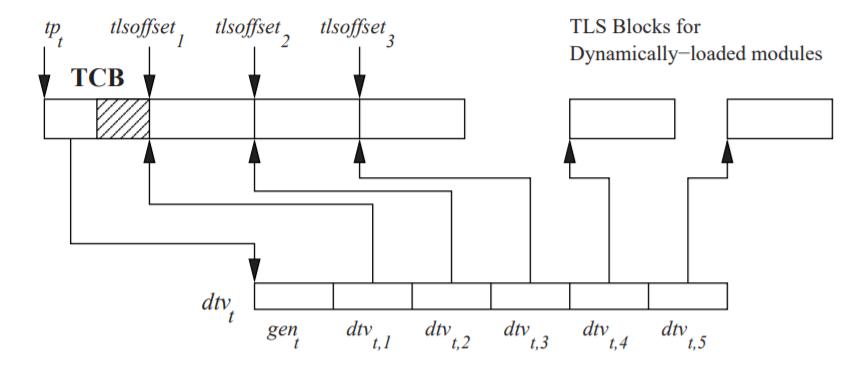
\includegraphics[scale=0.6]{slike/TLSModelV1.png}
	\end{center}
	\caption{TLS struktura podataka. Varijanta 1.}
	\label{fig:tls_model1}
\end{figure}

Na slici \ref{fig:tls_model1} je prikazan primer prve varijante \emph{TLS} strukture podataka. Nitni registar za nit \texttt{t} je označen sa \texttt{$tp_t$}. Početak  memorije svake niti je određen \emph{nitnim kontrolnim blokom \texttt{TCB}} (\emph{eng.~Thread Control Block}). Nitni registar pokazuje na nitni kontrolni blok, koji na pomeraju nula sadrži pokazivač na \emph{nitni dinamički vektor} \texttt{$dtv_t$} za tu određenu nit. Nitni dinamički vektor predstavlja niz koji sadrži informacije o podacima lokalnim za niti različitih učitanih modula. Memoriju lokalnu za nit u okviru jednog učitanog modula nazivamo \emph{TLS blok}. Ukoliko je modul inicijalno dostupan, tj. učitan u program prilikom pokretanja, element nitnog dinamičkog vektora pokazuje na fiksni pomeraj podataka lokalnog za tu nit u okviru tog modula. Ukoliko se modul dinamički učitava u program element dinamičkog nitnog vektora pokazuje na memoriju lokalnu za nit u okviru tog modula koji se učitava. \emph{TLS šablon} (\emph{eng.~template}) je sastavljen od svih \emph{TLS} blokova koji su učitani prilikom pokretanja procesa.

Na slici \ref{fig:tls_model1} nitni dinamički vektor \texttt{$dtv_t$} kao svoje prvo polje sadrži generacioni broj \texttt{$gen_t$} koji se koristi pri promeni veličine nitnog dinamičkog vektora i alokacije \emph{TLS} blokova. Ostala polja sadrže pokazivače na \emph{TLS} blokove za različite učitane module. \emph{TLS} blokovi za module koji se učitavaju pri pokretanju programa su smeštena direktno nakon \texttt{TCB} bloka i stoga ima arhitekturalno specifičan, fiksni pomeraj od adrese na nitni pokazivač. Za sve inicijalno dostupne module pomeraj svakog \emph{TLS} bloka, uz to i pomeraj \emph{TLS} promenljive, u odnosu na \texttt{TCB} mora biti fiksan nakon pokretanja programa.

Druga varijanta \emph{TLS} strukture podataka ima sličnu strukturu kao prva. Prikazana je na slici \ref{fig:tls_model2}. Jedina razlika je ta što nitni pokazivač pokazuje na nitni kontrolni blok za koji je nepoznata veličina i sadržaj. Negde svakako taj nitni kontrolni blok sadrži pokazivač na dinamički nitni vektor, ali nije navedeno gde. To je kontrolisano od strane mehanizma za izvršavanje programa.

\begin{figure}[h!]
	\begin{center}
		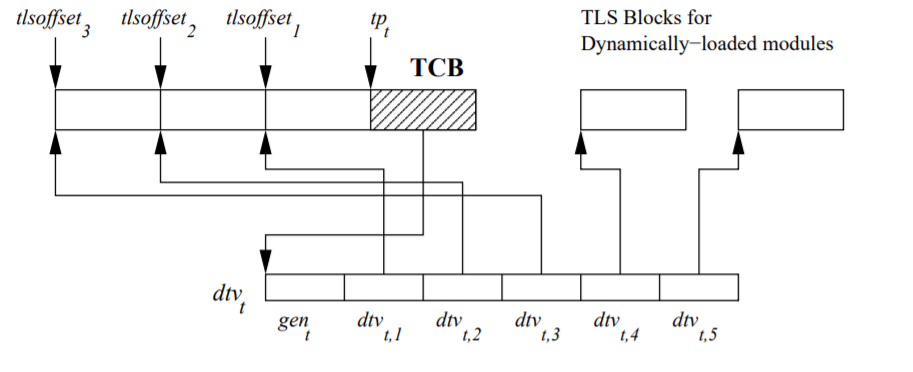
\includegraphics[scale=0.6]{slike/TLSmodelV2.png}
	\end{center}
	\caption{TLS struktura podataka. Varijanta 2.}
	\label{fig:tls_model2}
\end{figure}

U trenutku pokretanja programa \texttt{TCB}, zajedno sa dinamičkim nitnim vektorom, se kreira za glavnu nit. Pozicija tog \emph{TLS} bloka, za svaki pojedinačan modul, se računa koristeći arhitekturalno specifične formule, zasnovane na veličini i poravnanju \emph{TLS} bloka propisanih \emph{ABI}-jem za tu specifičnu procesorsku arhitekturu.

\section{Pokretanje i izvršavanje procesa}

Za programe koji koriste \emph{TLS} promenljive mehanizam operativnog sistema koji služi za pokretanje procesa mora podesiti memoriju za inicijalnu nit pre nego što preda kontrolu tog procesa drugim mehanizmima. Podrška za korišćenje \emph{TLS} promenljive u statičko povezanim programima je limitirana. Neke procesorske arhitekture (kao npr.~\emph{IA-64}) ne definišu uopšte statičko povezivanje. Neke druge platforme obeshrabruju korišćenje statičkog povezivanja pružanjem samo određenog broja funkcionalnosti. Rukovanje \emph{TLS} promenljivom u statičko povezanom programu je prosto, zbog postojanja samo jednog modula, tj.~samo taj program.

Zanimljiviji je slučaj rukovanja \emph{TLS} promenljivom u dinamičko povezanom programu. U ovom slučaju dinamički povezivač mora uključiti podršku za rukovanje takvih segmenata podataka. U nastavku teksta je opisano učitavanje i pokretanje dinamičkog koda.

Da bi se podesila memorija lokalna za nit, dinamički povezivač čita sve potrebne informacije o svakom modulu, i o njegovim \emph{TLS} blokovima, iz \texttt{PT\_TLS} polja tabele \emph{TLS} programskog zaglavlja prikazanog u tabeli \ref{tab:tls_prheader}. Informacije o svim modulima moraju biti prikupljene. Ovaj proces se ostvaruje koristeći povezanu listu čiji element sadrži:

\begin{itemize}
	\item pokazivač na \emph{TLS} inicijalizacionu sliku
	\item veličinu \emph{TLS} inicijalizacione slike
	\item \emph{TLS} pomeraj (\texttt{$tlsoffset_m$}) za module \texttt{m}
	\item fleg koji daje informaciju o tome da li modul koristi statički \emph{TLS} model
\end{itemize}

Ove informacije će biti proširene kada se učitaju dodatni dinamički moduli. Te informacije se koriste od strane standardne biblioteke za rukovanje nitima prilikom podešavanja \emph{TLS} blokova za novokreiranu nit.

Promenljiva unutar lokalnog prostora za nit, \emph{TLS}, je identifikovana po referenci na modul i pomeraju u okviru tog \emph{TLS} bloka. Ukoliko imamo strukturu podataka dinamički nitni vektor, možemo definisati referencu na neki modul kao ceo broj (\emph{eng.~integer}), počevši od broja \texttt{1}. To može biti korišćeno kao indeks u \texttt{$dtv_t$} nizu. Identifikacione brojeve koji svaki modul dobija određuje mehanizam izvršavanja programa, obično neki modul standardne biblioteke za rukovanje nitima. Samo izvršni fajl dobija fiksan broj, \texttt{1}, a svi ostali učitani moduli dobijaju različite brojeve.

Računanje specifične adrese neke \emph{TLS} promenljive je prosta operacija koja može biti izvršena ukoliko je programski prevodilac koji je preveo k\^{o}d korsitio varijantu 1 \emph{TLS} strukture podataka. Ali to ne može biti tako lako odrađeno u kodu koji je generisan od strane kompajlera za procesorske arhitekture koje koriste varijatnu 2 \emph{TLS} strukture podataka.
Umesto toga, definisana je funkcija \texttt{\_\_tls\_get\_addr()}, koja je prikazana u okviru listinga \ref{lst:ex1}.

\begin{lstlisting}[style=customc, label={lst:ex1}, caption={Implementacija funkcije \texttt{\_\_tls\_get\_addr()}.}]
void *
__tls_get_addr (size_t m, size_t offset)
{
  char *tls_block = dtv[thread_id][m];
  return tls_block + offset;
}

\end{lstlisting}

Smeštanje vektora \texttt{dtv[thread\_id]} u memoriju je arhitekturalno specifično. Sa \texttt{m} se označava identifikacioni broj modula, koji mu je dodeljen od strane dinamičkog punionca prilikom učitavanja. Korišćenje \texttt{\_\_tls\_get\_addr()} funkcije ima i dodatne prednosti kako bi se olakšala implementacija dinamičkog modela, gde je alokacija nekog \emph{TLS} bloka odložena do njegove prve upotrebe. Da bi se to podržalo potrebno je popuniti \texttt{dtv[thread\_id]} vektor sa specijalnom vrednošću kojom će biti prepoznate situacije kada je taj vektor trenutno prazan, tj.~da u datom trenutku određeni blok nije u upotrebi. To je omogućeno malom promenom u izvornom kodu \texttt{\_\_tls\_get\_addr()} funkcije koja je prikazana u okviru listinga \ref{lst:ex2}.\newpage

\begin{lstlisting}[style=customc, label={lst:ex2}, caption={Promena implementacije funkcije \texttt{\_\_tls\_get\_addr()}.}]
void *
__tls_get_addr (size_t m, size_t offset)
{
  char *tls_block = dtv[thread_id][m];
  if (tls_block == UNALLOCATED_BLOCK)
    tls_block = dtv[thread_id][m] = allocate_tls(m);
  return tls_block + offset;
}

\end{lstlisting}

Funkcija \texttt{allocate\_tls()} određuje memorijske zahteve \emph{TLS} modula \texttt{m} i inicijalizuje ga ispravno. Postoje dva tipa podataka: inicijalizovani i neinicijalizovani. Inicijalizovani podaci moraju biti kopirani iz inicijalizacione nitne slike, podešenih prilikom učitavanja modula \texttt{m}. Neinicijalizovani podaci se postavljaju na vredosti \texttt{0}. Primer implementacije funkcije \texttt{allocate\_tls()} je prikazan u okviru listinga \ref{lst:exal}.

\begin{lstlisting}[style=customc, label={lst:exal}, caption={Implementacija funkcije \texttt{allocate\_tls()}.}]
void *
allocate_tls (size_t m)
{
  void *mem = malloc (tlssize[m]);
  memset (memcpy (mem, tlsinit_img[m], tlsinit_size[m]), '\0',
          tlssize[m] - tlsinit_size[m]);
  return mem;
}

\end{lstlisting}

\texttt{tlssize[m]}, \texttt{tlsinit\_size[m]} i \texttt{tlsinit\_img[m]} su poznati nakon učitavanja modula \texttt{m}. Primetimo da se ista inicijalizaciona slika \texttt{tlsinit\_img[m]} koristi za sve niti modula, bilo kada da se one kreiraju. Novonapravljena nit ne nasleđuje podatke od svog roditelja (\emph{eng.~parent}), već dobija samo kopiju inicijalnih podataka.

\section{TLS modeli pristupa}

Svako referisanje \emph{TLS} promenljive prati jedan od dva modela pristupa: dinamički ili statički. Različite arhitekture ABI-jem propisuju koji od modela pristupa će koristiti kao podrazumevani. Postoje različiti modeli pristupa, a četiri najpoznatija su opisana u nastavku teksta.

\subsection{Generalni dinamički TLS model}

Generalni model pristupa \emph{TLS} promenljivoj dozvoljava referisanje svih \emph{TLS} promenljivih, bilo da je to iz deljene biblioteke ili dinamičkog izvršnog fajla. Ovaj model takođe podržava odloženo alociranje \emph{TLS} bloka do trenutka kada se prvi put taj blok referiše iz specifične niti.

\subsection{Lokalni dinamički TLS model}

Lokalni dinamički model pristupa \emph{TLS} promenljivoj predstavalja optimizaciju generalnog dinamičkog modela. Programski prevodilac može odrediti da je neka promenljiva definisana samo lokalno, ili zaštićeno (\emph{eng.~protected}) u objektu koji je napravljen u programu. U tom slučaju, programski prevodilac daje instrukcije linkeru da statički poveže dinamički \emph{TLS} pomeraj i da korsiti ovaj model. Iz tog razloga predstavlja hibridnu kombinaciju statičkog i dinamičkog modela pristupa, te prema tome predstavlja model koji diže performanse u odnosu na generalni dinamički model. Samo jedan poziv \texttt{tls\_get\_addr()} po funkciji je potreban za određivanje adrese \texttt{$dtv_{0,m}$}.

\subsection{Statički TLS model sa dodeljenim pomerajima}

Ovaj model pristupa dopušta referisanje samo na one \emph{TLS} promenljive koje su dostupne kao deo inicijalnog statičkog \emph{TLS} šablona. U ovom modelu, relativni pomeraj pokazivača na nit date promenljive \texttt{x} je smešten u polju globalne tabele sa pomeraijma (\emph{eng.~Global offset table-GOT}) za promenljivu \texttt{x}.

Deljene biblioteke uobičajeno koriste dinamički model pristupa, jer statičkim modelom mogu referisati samo na određeni broj \emph{TLS} promenljivih.

\subsection{Statički TLS model}

Ovaj model pristupa dopušta referisanje samo na one \emph{TLS} promenljive koje su dostupne kao deo \emph{TLS} bloka od tog dinamičkog izvršnog fajla. Linker računa relativni pomeraj pokazivača na nit statički, bez potrebe za dinamičkim realokacijama ili dodatnih inforamcija iz \emph{GOT}-a. Ovaj model pristupa ne dopušta referisanje \emph{TLS} promenljivih izvan tog dinamički povezanog izvršnog fajla.

\chapter{Implementacija rešenja}
\label{chp:Implementacija}

\emph{TLS} mehanizam može biti različito implementiran za različite procesorske arhitekture. \emph{TLS} promenljiva se može smeštati u posebne registre, u određene delove memorije itd. \emph{GNU GDB} alat mora poznavati sve arhitekturne razlike i anulirati ih na neki način. Implementacija realizovanog rešenja za proširenje alata se upravo i zasniva na prethodnoj činjenici. Zbog toga su detaljno istražene implementacije \emph{TLS} mehanizma raznih arhitektura, kako u funkcijama \emph{GNU C} biblioteke (poznatije kao \emph{glibc}) \cite{GLIBC}, tako i karakteristike koje su \emph{ABI}-jem propisane.

Poboljšanje alata koje je uspešno realizovano se odnosi na verziju \emph{Multiarch}. Izvorni k\^{o}d alata i instrukcije za prevođenje i upotrebu debagera sa pobljšanjem za pristupanje vrednosti \emph{TLS} promenljive se može pronaći na strani \cite{GITMOJ}. Ukoliko je program koji je učitan u \emph{Multiarch GNU GDB} alat iste arhitekture kao arhitektura domaćina, zadržava se način čitanja vrednosti \emph{TLS} promenljive kao u slučaju \emph{GNU GDB} debagera arhitekture domaćina, jer je ta funkcionalnost već implementirana. Rešenje obuhvata arhitekture procesora \emph{MIPS}, \emph{ARM}, \emph{AARCH64}, \emph{i386} i \emph{PowerPC}. Kao odgovor na komentare \emph{GNU} zajednice razvijeno je i alternativno rešenje koje je takođe opisano u nastavku teksta.

Treba napomenuti da je u razvoju i rešenje od strane programera iz kompanije \emph{Red Hat} \cite{REDHAT} u vidu projekta \emph{Infinity} \cite{Infinity}. Taj projekat ima ideju da obuhvati rešenja za razne probleme o debagovanju niti, ne samo obradu \emph{TLS} mehanizma. Prednost rešenja koji se predstavlja u ovom master radu je što je cela funkcionalnost prepuštena samom \emph{GNU GDB} debageru, te nema potrebe za instalacijom ili prevođenjem eksternih projekata, čime se dobija na uštedi korisničkog napora pri korišćenju debagera.

\section{Detalji implementacije}

U nastavku teksta opisani su detalji implementacije poboljšanja debagera.

\subsection{Izmena sistema izgradnje alata}

Fajlovi \emph{gdb/configure} i \emph{gdb/Makefile.in} su zaduženi za izgradnju alata. U najopštijem slučaju na \emph{UNIX}-olikim operativnim sistemima, \emph{configure} skripta je zadužena za pravljenje konačnog \emph{Makefile} od ulaznog \emph{gdb/Makefile.in}.

Izvorni k\^{o}d koji u sebi sadrži funkcije za čitanje \emph{TLS} promenljive (\emph{gdb/linux-thread-db.c}) se prevodio samo za domaćinsku verziju \emph{GNU GDB} debagera, pa stoga u proširenje za \emph{Multiarch} \emph{GNU GDB} takođe treba uvrstiti izmenu u pomenutom fajlu prilikom prevođenja. Pored toga, postojeće funkcije koje su zadužene za pristupanje vrednosti \emph{TLS} promenljivih je trebalo izmeniti te je u projekat dodat direktorijum \emph{gdb/glibc-dep/} koji sadrži funkcije koje barataju sa \emph{TLS} mehanizmom različite procesorske arhitekture od arhitekture domaćina. Da bi se ti fajlovi prevodili samo u slučaju \emph{Multiarch} verzije definisan je makro pod imenom \texttt{CROSS\_GDB} koji se definiše prilikom kreiranja \emph{Makefile}. Da bi se ispratila konvencija pisanja skripti za izgradnju alata, u direktorijum \emph{gdb/config/} je dodat fajl \emph{glibc.mh} koji definiše spisak objektnih fajlova koji služe sa pristupanje vrednosti \emph{TLS} promenljive u tom slučaju i takođe u tom fajlu se definiše gore pomenuti makro \texttt{CROSS\_GDB}.

Sadržaj \emph{gdb/config/glibc.mh} fajla je prikazan na listingu \ref{lst:conf2}.
\begin{lstlisting}[label={lst:conf2}, caption={Sadržaj \emph{gdb/config/glibc.mh} fajla.}]
# GLIBC fragment comes in here
GLIBCFILES = td_symbol_list.o \
       fetch-value.o gdb_td_ta_new.o \
       td_thr_tlsbase.o td_thr_tls_get_addr.o \
       td_ta_map_lwp2thr.o native_check.o
INTERNAL_CFLAGS += -DCROSS_GDB
\end{lstlisting}

Da bi sadržaj iz novokreiranog \emph{gdb/config/glibc.mh} fajla bio ispisan u krajnji \emph{Makefile} trebalo je uvesti promenljivu koja proverava da li je u prilikom navođenja opcija \emph{gdb/configure} skripti navedena opcija \emph{--enable\_targets}, koja zapravo označava da korisnik ima nameru da alat prevede kao \emph{Multiarch} verziju. Vrednost promenljive \texttt{cross\_makefile\_frag} u \emph{gdb/configure} skripti postaje putanja do \emph{gdb/config/glibc.mh} fajla ukoliko je pomenuta opcija navedena, a u suprotnom ona ostaje prazna.

Deo koda u \emph{gdb/configure} skripti kojim se to postiže je prikazan na listingu \ref{lst:conf}.
\begin{lstlisting}[label={lst:conf}, caption={Izmena \emph{gdb/configure} fajla.}]
if test "${gdb_native}" = "no" ||
   test "${enable_targets}" != ""; then
  cross_makefile_frag=${srcdir}/config/glibc.mh
else
  cross_makefile_frag=/dev/null
fi
\end{lstlisting}

\subsection{Implementacija funkcija za pristupanje TLS promenljivoj}

U direktorijumu \emph{gdb/glibc-dep/} se nalazi srž funkcionalnosti čitanja vrednosti \emph{TLS} promenljive iz datoteke jezgara sa platformi drugih procesorskih arhitektura. Kako standardna C biblioteka već ima implementirane svaku arhitekturalnu zavisnost u vezi \emph{TLS} mehanizma za svaku procesorsku arhitekturu podržanu u alatu \emph{GNU GDB}, potrebno je na neki način izopštiti tu funkcionalnost iz same biblioteke unutar alata. Preciznije, za baratanjem nitima \emph{GNU GDB} koristi \emph{libthread\_db} biblioteku iz standardne biblioteke. Funkcije \texttt{td\_ta\_new()}, \texttt{td\_thr\_tls\_get\_addr()} i \texttt{td\_th\_tlsbase()}, koje se služe za pristupanje \emph{TLS} promenljivama, očekuju da se na arhitekturi domaćina prirodno barata sa programima iste arhitekture. Izbegavanje modifikacije \emph{libthread\_db} biblioteke moguće je tako što se pomenute funkcije implementiraju u \emph{GNU GDB}-u, na isti način kao u \emph{glibc} biblioteci, prilikom čega se sve arhitekturno zavisne vrednosti promenljivih i makroa koje primaju te funkcije postave na vrednosti koje bi trebalo da imaju u slučaju da je ta ciljna arhitektura zapravo arhitektura domaćina.

Prvi korak ovog dela implementacije je izmeštanje funkcija iz standardne biblioteke unutar GDB projekta. Unutar \emph{gdb/glibc-dep/} je kreiran direktorijum \emph{nptl\_db} koji sadrži pomenute funkcije. Zapravo, ukoliko alat koristi bilo koju verziju standardne biblioteke do \emph{2.22} funkcije iz \emph{nptl\_db} nisu ni potrebne za pristupanje vrednosti \emph{TLS} promenljive. Sve potrebne informacije za pristupanje vrednosti \emph{TLS} promenljive se mogu pročitati iz same datoteke jezgra. Ukoliko alat koristi verziju standardne biblioteke 2.22 i ili veću, funckcije iz \emph{nptl\_db} direktorijuma su neophodne kako bi se anulirale novonastale izmene prilikom baratanja \emph{TLS} mehanizmom. Ta funkcionalnost je dodata u funkciji \texttt{gdb\_td\_thr\_tlsbase()} koja je dodata u fajl \texttt{gdb/glibc-dep/nptl\_db/td\_thr\_tlsbase.c}.
Sve funkcije koje bi trebalo da emuliraju ponašanje \emph{TLS} funkcija standardne biblioteke koje su dodate u projekat \emph{GNU GDB} imaju prefiks u imenu \texttt{gdb\_}. Npr.~GDB pandam funckiji \texttt{td\_ta\_new()} je \texttt{gdb\_td\_ta\_new()}. Pomenuta funkcija je promenjena da bi alat \emph{GNU GDB} imao inforamciju o tačnoj verziji standardne biblioteke koju je program koji se debaguje koristio na platformi na kojoj se izvršavao, jer kao što je napomenuto od verzije 2.22 \emph{TLS} promenljiva se drugačije čita. Nije novo da za debagovanje višenitnih programa \emph{GNU GDB} debagerom, čak i upotrebom domaćinske verzije, je neophodno da \emph{GNU GDB} koristi istu veriziju \emph{libthread\_db} biblioteke kao i program koji se debaguje. To znači ako je program preveden sa verzijom \emph{2.x} standardnom bibliotekom, alat mora korsiti istu verziju \emph{2.x} tokom svog debagovanja. To se postiže eksplicitnim navođenjem putanje do \emph{libthread\_db} biblioteke komandom \texttt{set libthread-db-search-path}. Ukoliko se verzije \emph{libthread\_db} biblioteke ne poklapaju debager će ispisati upozorenje.

Takođe u \texttt{gdb\_td\_ta\_new()} funkiji se poziva funkija \texttt{init\_target\_dep\_constants()}, zadužena za inicijalizaciju arhitekturalno zavisnih osobina o \emph{TLS} mehanizmu.

Deo kojim se različite osobine inicijalizuju za arhitekture \emph{MIPS} i \emph{ARM} u funkciji \texttt{init\_target\_dep\_constants()} je prikazan na listingu \ref{lst:izmenaBFD}.
\begin{lstlisting} [style=customc, label={lst:izmenaBFD}, caption={Inicijalizacija arhitekturalno yavisnih osobina o TLS.}]
case bfd_arch_mips:
  tls_tcb_at_tp = 0;
  tls_dtv_at_tp = 1;
  forced_dynamic_tls_offset = -2;
  no_tls_offset = -1;
  tcb_alignment = 16;
  break;
case bfd_arch_arm:
  tls_tcb_at_tp = 0;
  tls_dtv_at_tp = 1;
  forced_dynamic_tls_offset = -2;
  no_tls_offset = -1;
  tcb_alignment = 0;
  break;
\end{lstlisting}
U ovom konkretnom slučaju sve osobine \emph{TLS} mehanizma su identične, osim poravnanja nitnog kontrolnog bloka.

Funkcija \texttt{native\_check()} definisana u fajlu \emph{gdb/glibc-dep/native-check.c} daje informaciju da li se \emph{Multiarch} verzijom alata debaguje program domaćinske arhitekture. Ako je to slučaj, pristupanje vrednosti \emph{TLS} promenljive se vrši kao do sada uz pomoć funkcija iz standardne C biblioteke. Ukoliko to nije slučaj, pozovaju se novokreirane funkcije iz direktorijuma \emph{gdb/glibc-dep/}.

Cela funkcionalnost se zapravo dodaje u \emph{gdb/linux-thread-db.c} fajl u funkciju koja je zadužena za pristupanje vrednosti \emph{TLS} promenljive. Izmena nije direktno u funkciji \texttt{thread\_db\_get\_thread\_local\_address} koja vraća adresu \emph{TLS} promenljive. Naime, promena je izvedena u funkciji \texttt{try\_thread\_db\_load\_1()} koja uspostavlja konekciju između alata GDB i \emph{libthread\_db} biblioteke. Promenjeni su pokazivači na \emph{TLS} funkcije u slučaju nedomaćinskih datoteka jezgara.

Deo koda koji implementira pomenutu funkcionalnost je prikazan na listingu \ref{lst:izmenaTLS}.
\begin{lstlisting} [style=customc, label={lst:izmenaTLS}, caption={Postavljanje \emph{callback} funkcija za nedomaćinske arhitekture.}]
#ifdef CROSS_GDB
 if (native_check(arch) != 0) {
  info->td_thr_tls_get_addr_p=gdb_td_thr_tls_get_addr;
  info->td_thr_tlsbase_p=gdb_td_thr_tlsbase;
 } else {
  //if it's host we want to keep old way of counting tls address
  TDB_DLSYM (info, td_thr_tls_get_addr);
  TDB_DLSYM (info, td_thr_tlsbase);
 }
#else
  TDB_DLSYM (info, td_thr_tls_get_addr);
  TDB_DLSYM (info, td_thr_tlsbase);
#endif
\end{lstlisting}
Iako je u pitanju \emph{Multiarch} verzija alata, ako je datoteka jezgra kreirana na domaćinskoj platformi zadržava se normalno pristupanje \emph{TLS} mehanizma.

\section{Alternativno rešenje}

Drugi način implementacije je modifikacija \emph{libthread\_db} funkcija eksplicitno u standardnoj biblioteci, modifikujući ih tako da rade sa različitim arhitekturama. Naime, formula koja služi za pristupanje \emph{TLS} promenljive se računala u vremenu prevođenja biblioteke, sada bi se računala u vremenu izvršavanja programa, i u zavisnosti od arhitekture promenljive koje učestvuju u pomenutoj formuli će dobiti odgovarajuće vrednosti. Ukoliko se radi o programu arhitekture domaćina u funkciji  \texttt{td\_ta\_new()} promenljive dobijaju vrednosti koje odgovaraju arhitekturi domaćina, dok ako se radi o programu ciljne arhitekture, tj. različite od arhitekture domaćina, iz \emph{GNU GDB}-a će biti pozvana nova funckija u standardnoj biblioteci \texttt{td\_ta\_init\_target\_consts()} koja će postaviti vrednosti promenljivih koje odgovaraju ciljnoj arhitekturi. Ideja je upisati ove vrednosti u datoteku jezgra na ciljnoj arhitekturi i kasnije ih pročitati na arhitekturi domaćina korišćenjem \emph{GNU GDB} debagera. U ovom slučaju izmena u samom \emph{GNU GDB}-u bi bila minorna, te zahteva samo proveru da li je učitani program arhitekture domaćina ili ne, i u zavisnosti od toga se poziva \texttt{td\_ta\_init\_target\_consts()} ili ne. Ovo rešenje je nastalo kao odgovor na komentare \emph{GNU} zajednice na predhodno rešenje. Izmena standardne biblioteke se može pronaći na strani \cite{GLIBCPATCH}.

\section{Čitanje/pisanje datoteke jezgra za procesorsku arhitekturu MIPS}

Kako bi funkcionalnost bila moguća za svaku podržanu procesorsku arhitekturu, potrebno je da alat \emph{GNU GDB} ima potpunu podršku za čitanje informacija iz datoteka jezgara. Podrška je za sve arhitekrure potpuna, ali u trenutku razvoja ove funkcionalnosti uočeno je da alat nema potpunu podršku za čitanje identifikacionog broja procesa (eng.~\emph{Process ID}) iz datoteke jezgra za arhitekture \emph{MIPS}, neophodnog za pristupanje bazičnih informacija o nitima. Koristeći komandu alata \texttt{gcore} moguće je kreirati datoteku jezgra i sa korisničkog nivoa, gde je takođe uočeno da alat nema potpunu podršku za ispisivanje nekih informacija o procesu za procesorsku arhitekturu \emph{MIPS}. Da bi podrška za \emph{TLS} promenljive bila potpuna i za arhitekturu \emph{MIPS}, implementirani su i uočeni nedostaci. Ova implementacija je privaćena od strane \emph{GNU} zajednice i ušla je u izvršnu verziju alata 8.0.0.

Deo izvornog koda (u fajlu \emph{bfd/elf32-mips.c}) izmene za čitanje informacija o procesu iz datoteke jezgra je prikazan na listinigu \ref{lst:izmenaBFD2}. Bitna informacija za čitanje vrednosti \emph{TLS} promenljive je identifikacioni broj procesa. Bez izmene prikazane u listingu \ref{lst:izmenaBFD2} to ne bi bilo moguće. \newpage
\begin{lstlisting} [style=customc, label={lst:izmenaBFD2}, caption={Deo izmene za čitanje informacija o procesu iz datoteke jezgra.}]

case 128:                /* Linux/MIPS elf_prpsinfo */
  elf_tdata (abfd)->core->pid
   = bfd_get_32 (abfd, note->descdata + 16);
  elf_tdata (abfd)->core->program
   = _bfd_elfcore_strndup (abfd, note->descdata + 32, 16);
\end{lstlisting}

Ukoliko se koristi datoteka jezgra generisana iz korisničkog nivoa koristeći debager, bez upisivanja u nju informacija o procesu (kao npr.~identifikacioni broj procesa) čitanje vrednosti \emph{TLS} promenljive nije moguće. Deo izvornog koda (u fajlu \emph{bfd/elf32-mips.c}) izmene za pisanje informacija o procesu u datoteku jezgra je prikazan na listinigu \ref{lst:izmenaBFD3}.
\begin{lstlisting} [style=customc, label={lst:izmenaBFD3}, caption={Deo izmene za pisanje informacija o procesu u datoteku jezgra.}]
  ...
    case NT_PRSTATUS:
      {
       char data[256];
       va_list ap;
       long pid;
       int cursig;
       const void *greg;

       va_start (ap, note_type);
       memset (data, 0, 72);
       pid = va_arg (ap, long);
       bfd_put_32 (abfd, pid, data + 24);
       cursig = va_arg (ap, int);
       bfd_put_16 (abfd, cursig, data + 12);
       greg = va_arg (ap, const void *);
       memcpy (data + 72, greg, 180);
       memset (data + 252, 0, 4);
       va_end (ap);
       return elfcore_write_note (abfd, buf, bufsiz,
                                  "CORE", note_type, data, sizeof (data));
      }
  ...
\end{lstlisting}

Primeri izvornog koda izmena su prikazani samo za 32-bitnu verziju arhitekture \emph{MIPS}. Napomenimo da izmena obuhvata i 64-bitnu verziju procesorske arhitekture \emph{MIPS}.

\section{Testiranje}

Faza testiranja je jako važan deo životnog ciklusa razvoja softvera, te je veliki značaj dat ovoj sekvenci. Testiranje je izvršeno na raznim verzijama procesorskih arhitektura \emph{ARM} i \emph{MIPS}.

Takođe, implementirani su \emph{DejeGNU} \cite{DejaGNU} testovi koji testiraju pristupanje vrednosti \emph{TLS} promenljive iz datoteka jezgara raznih arhitektura. Zbog prirode problema koji se testira datoteke jezgra su generisane na različitim platformama i kompresovane zajedno sa izvršnim fajlom u \emph{gdb/testsuite/gdb.multi/}, te se prilikom izvršavanja konkretnih testova ti fajlovi raspakuju i učitavaju u debager. Testovi obuhvataju izvršne fajlove sa \emph{TLS} mehanizmom generisanih koristeći \emph{2.19} i \emph{2.22} verzije standardne biblioteke.

Komanda alata kojom pokrećemo testove, ukoliko smo pozicionirani u direktorijumu gde je alat izrađen je prikazana na listingu \ref{lst:makec}.

\begin{lstlisting} [style=BashInputStyle, label={lst:makec}, caption={Komanda za pokretanje testova.}]
make check
\end{lstlisting}

Pre izmene koja dodaje \emph{TLS} funkcionalnost, rezultati izvršavanja testova \emph{Multiarch GNU GDB} verzije debagera je prikazana na listingu \ref{lst:tst}

\begin{lstlisting} [style=BashInputStyle, label={lst:tst}, caption={Rezultati izvršavanja testova.}]
		=== gdb Summary ===
		# of expected passes		33715
		# of expected failures		196
		# of known failures		    66
		# of unresolved testcases	5
		# of untested testcases		67
		# of unsupported tests		219
\end{lstlisting}
 
Posle izmene koja dodaje \emph{TLS} funkcionalnost, rezultati izvršavanja testova \emph{Multiarch GNU GDB} verzije debagera je prikazana na listingu \ref{lst:tst2}.

\begin{lstlisting} [style=BashInputStyle, label={lst:tst2}, caption={Rezultati izvršavanja testova.}]
		=== gdb Summary ===
		# of expected passes		33718
		# of expected failures		196
		# of known failures		    66
		# of unresolved testcases	5
		# of untested testcases		67
		# of unsupported tests		219
\end{lstlisting}

Rezultati testiranja prikazani u listinzima \ref{lst:tst} i \ref{lst:tst2} pokazuju da nema regresije prilikom testiranja alata. Tri testa koja dodatno prolaze jesu testovi koji su dodati izmenama koji se opisuju u ovom radu. Dodati testovi sadrže primere čitanja vrednosti \emph{TLS} promenljive, koji se mogu naći u realnoj upotrebi.

\section{Upotreba alata}

Da bi \emph{GNU GDB} uspešno koristio naprednije tehinke analize višenitnih programa, uključujući i analizu \emph{TLS} mehanizma, potrebno je da mu se prosledi putanja do \emph{libthread\_db} biblioteke koja pripada istoj verziji standardne biblioteke kao i program koji se debaguje. To isto važi i za \emph{Multiarch GNU GDB} verziju alata. Nakon toga potrebno je zadati putanju do biblioteka koje je program koristio na tom uređaju sa ugrađenim računarom na kome se program izvršavao. Primetimo da te biblioteke pripadaju toj ciljanoj platformi. Debager neće izvršavati program koji se debaguje, već će samo rekonstruisati sliku stanja tog procesa kada je neočekivano prekinuo sa radom, čitajući informacije iz datoteke jezgra i deljenih biblioteka.


Izvorni kod višenitnog programa koji se debaguje u primeru je napisan u programskom jeziku \emph{C} i prikazan je na listingu \ref{lst:ctst}.\newpage

\begin{lstlisting} [style=customc, label={lst:ctst}, caption={Višenitni test primer napisan u C kodu.}]
#include <stdio.h>
#include <stdlib.h>
#include <unistd.h>
#include <pthread.h>

__thread int foo=0xdeadbeef;
pthread_t threads[5];

void* thread(void *e) {
  int *i = (int*)e;
  foo+=*i;
  printf("foo is %x\n", foo);
  sleep(10);
  return (void*)0;
}   

int main()
{
  printf("init %x\n", foo);
  int i;
  for (i=0; i<5; i++) {
    pthread_create(&threads[i], NULL, thread, &i);
  }

  for (i=0; i<5; i++) {
    pthread_join(threads[i], NULL);
  }

  sleep(5);
  abort();
}

\end{lstlisting}

Korišćenje debagera pre implementacije čitanja vrednosti \emph{TLS} promenljive iz datoteke jezgra generisane na uređaju sa ugrađenim računarom arhitekture \emph{MIPS} je prikazano na listingu \ref{lst:gdbkom}.\newpage

\begin{lstlisting} [style=BashInputStyle, label={lst:gdbkom}, caption={Korišćenja debagera pre implementacije.}]
(gdb) add-auto-load-safe-path /home/glibc/build_22/INSTALL/lib
(gdb) set libthread-db-search-path /home/glibc/build_22/INSTALL/lib
(gdb) set solib-search-path ~/master_examples/mips_arch
(gdb) file ~/master_examples/mips_arch/example222 
Reading symbols from ~/master_examples/mips_arch/example...done.
(gdb) core-file ~/master_examples/mips_arch/core
[New LWP 21808]
[New LWP 21813]
[New LWP 21810]
[New LWP 21809]
[New LWP 21811]
[New LWP 21812]
[Thread debugging using libthread_db enabled]
Using host libthread_db library "/home/glibc/build_22/INSTALL/lib/libthread_db.so.1".
Core was generated by `./example'.
Program terminated with signal SIGABRT, Aborted.
#0  0x00000000 in ?? ()
[Current thread is 1 (LWP 21808)]
(gdb) p/x foo
Cannot find user-level thread for LWP 21808: generic error
\end{lstlisting}

\emph{Prvom i drugom komandom alata (linije 1 i 2) se podešavaju putanje do standardne biblioteke za debagovanje niti koja ima istu verziju kao i izvršni fajl koji se debaguje. Trećom komandom (linija 3) se zadaje putanja do deljenih biblioteka koje je izvršni fajl koji se debaguje korsitio na uređaju sa ugrađenim računarom. Četvrta komanda (linija 4) učitava izvršni fajl koji se debaguje. Petom komandom (linija 6) se učitava datoteka jezgra koja je generisana prilikom neočekivanog prekidanja izvršavanja fajla koji se debaguje. Poslednjom komandom (linija 19) se bezuspešno pokušava čitanje vrednosti \emph{TLS} promenljive.}

Korišćenje debagera nakon implementacije čitanja vrednosti \emph{TLS} promenljive iz datoteke jezgra generisane na nekom uređaju sa ugrađenim računarom je prikazano na listingu \ref{lst:gdbkom2}.\newpage

\begin{lstlisting} [style=BashInputStyle, label={lst:gdbkom2}, caption={Korišćenja debagera posle implementacije.}]
(gdb) add-auto-load-safe-path /home/glibc/build_22/INSTALL/lib
(gdb) set libthread-db-search-path /home/glibc/build_22/INSTALL/lib
(gdb) set solib-search-path ~/master_examples/mips_arch
(gdb) file ~/master_examples/mips_arch/example222 
Reading symbols from ~/master_examples/mips_arch/example...done.
(gdb) core-file ~/master_examples/mips_arch/core
[New LWP 21808]
[New LWP 21813]
[New LWP 21810]
[New LWP 21809]
[New LWP 21811]
[New LWP 21812]
[Thread debugging using libthread_db enabled]
Using host libthread_db library "/home/glibc/build_22/INSTALL/lib/libthread_db.so.1".
Core was generated by `./example'.
Program terminated with signal SIGABRT, Aborted.
#0  0x00000000 in ?? ()
[Current thread is 1 (LWP 21808)]
(gdb) p/x foo
$1 = 0xdeadbeef
\end{lstlisting}

\emph{Prvom i drugom komandom alata (linije 1 i 2) se podešavaju putanje do standardne biblioteke za debagovanje niti koja ima istu verziju kao i izvršni fajl koji se debaguje. Trećom komandom (linija 3) se zadaje putanja do deljenih biblioteka koje je izvršni fajl koji se debaguje korsitio na uređaju sa ugrađenim računarom. Četvrta komanda (linija 4) učitava izvršni fajl koji se debaguje. Petom komandom (linija 6) se učitava datoteka jezgra koja je generisana prilikom neočekivanog prekidanja izvršavanja fajla koji se debaguje. Poslednjom komandom (linija 19) se uspešno čita vrednosti \emph{TLS} promenljive.}

% ------------------------------------------------------------------------------
\chapter{Zaključak}
% ------------------------------------------------------------------------------

Otkrivanje grešaka u višenitnim programima je veoma teško, u nekim slučajevima gotovo nemoguće, bez korišćenja debagera. Analizom višenitnih programa koristeći debager može se uštedeti dosta vremena. Posebno je teško analizirati rad programa na uređajima sa ugrađenim računarima. Često takvi uređaji nemaju dovoljno memorije da bi bilo moguće pokrenuti na njima debager. Učitavanje datoteke jezgra u debager na ličnim računarima je nekada jedina moguća opcija. Važno je da mogućnosti debagera prilikom takvih analiza budu što je moguće potpunije.

U ovom radu je prikazan uvod u debag informacije i rad debagera u opštem slučaju. Pored opisa formata debag informacija \emph{DWARF}, u radu je dat kratak uvod o formatu izvršnih fajlova \emph{ELF}. U radu je takođe naveden detaljan opis implementacije \emph{TLS} mehanizma, kako hardverski tako i softverski deo.

Funkcionalnost debagera prilikom čitanja vrednosti promenljive lokalne za nit iz datoteke jezgra generisane na uređaju sa ugrađenim računarom podiže kvalitet debagera. U radu su opisana dva moguća rešenja i njihove implementacije. Oba rešenja su poslata \emph{GNU} zajednici i u toku je pregled i analiza implementacije, čija se diskusija može videti na \cite{TLSPatch}. I prvi i drugi način imaju svoje prednosti i mane. Mana prvog načina jeste ta što svaka promena arhitekturno zavisnih vrednosti promenljivih koje učestvuju u računanju lokacije \emph{TLS} promenljive u \emph{glibc}-u zahteva izmenu i u \emph{GNU GDB}-u što dodatno otežava održavanje koda. Drugi način zahteva izmene i u izvornom kodu \emph{GNU GDB}-a i \emph{glibc}-a, ali ukoliko želimo da na sistemima arhitekture domaćina baratamo sa programima koji su prevedeni i izvršavani na nekim ciljnim arhitektura, što je za arhitekturu domaćina neprirodno, kompromisi jesu neophodni.

Kao mogući pravac poboljšanja rada, planirano je rešenje koje ne zavisi od standardne biblioteke. Ta zavisnost bi, uz pomoć upisivanja dodatnih informacija u datoteku jezgra, bila zaobiđena. Da bi se to omogućilo potrebne su promene u jezgru operativnih sistema prilikom generisanja datoteke jezgra.

% ------------------------------------------------------------------------------
% Literatura
% ------------------------------------------------------------------------------
\literatura

% ==============================================================================
% Završni deo teze i prilozi
\backmatter
% ==============================================================================

% ------------------------------------------------------------------------------
% Biografija kandidata
\begin{biografija}
Đorđe Todorović (\emph{Užice, 12. Avgust 1993.}) Rođen je u Užicu. Završio je Gimnaziju u Požegi, Informatički smer, 2012.~godine i iste godine upisao Matematički fakultet u Beogradu. 2016. godine je završio osnovne studije Matematičkog fakulteta i iste upisao master studije. Položio je sve ispite master studija u septembru 2018. godine. Od novembra 2015. pa do sada radi kao inženjer u Naučno-istraživačkom institutu RT-RK. Do sada je objavio nekoliko radova iz oblasti debagera i generisanja debag informacija od strane programskih prevodilaca. Na temu opisanu u master radu je objavio rad na konferenciji TELFOR \cite{TELFOR}. Trenutno radi na LLVM projektu, tačnije na poboljšanju tog prevodioca prilikom generisanja debag informacija.

Radovi:
\begin{enumerate}
	\item \emph{Ananthakrishna Sowda, Đorđe Todorović, Nikola Prica i Ivan Baev: Improving Debug Information in LLVM to Recover Optimized-out Function Parameters, 2019 European LLVM developers' Meeting (Brussels, Belgium)}
	\item \emph{Đorđe Todorović i Nikola Prica: Debug info in optimized code - how far can we go? (Improving LLVM debug info with function entry values), 2019 FOSDEM (Brussels, Belgium)}
	\item \emph{Ananthakrishna Sowda, Đorđe Todorović, Nikola Prica i Ivan Baev: Improving Debug Information in LLVM to Recover Optimized-out Function Parameters, 2018 Bay Area LLVM Developers' Meeting (San Jose, USA)}
	\item \emph{Nikola Prica, Đorđe Todorović i Petar Jovanović: Improving debug information generation inside LLVM compiler, 2018 Conference for electronics, communication, computing, automatizing and nuclear technique (Kladovo, Serbia)}
	\item \emph{Đorđe Todorović, Nikola Prica, Petar Jovanović i Nemanja Popov: Improvement Of GNU GDB For Analyzing TLS Variable From Core file Of Target Architecture, publication description, 2017 Telecommunications forum TELFOR (Belgrade, Serbia)}
\end{enumerate}

\end{biografija}
% ------------------------------------------------------------------------------

\end{document}